\documentclass{fenicsmanual}

\renewcommand{\P}{{\mathbb P}}

\begin{document}

\fenicstitle{UFC Specification and User Manual}
\fenicsauthor{Martin Sandve Aln\ae{}s, Hans Petter Langtangen, \\
Anders Logg, Kent-Andre Mardal and Ola Skavhaug}
\fenicspackage{\textbf{\textsf{UFC}}}{ufc}

\maketitle

\rhead{}

%% This chapter is common to the DOLFIN and FFC manuals.

\addcontentsline{toc}{chapter}{About this manual}
\chapter*{About this manual}

This manual is currently being written. A first version of this manual
should be ready sometime in the fall of 2005.

%------------------------------------------------------------------------------
\section*{Intended audience}

This manual is written both for the beginning and the advanced user.
There is also some useful information for developers. More advanced topics
are treated at the end of the manual or in the appendix.

%------------------------------------------------------------------------------
\section*{Typographic conventions}

\begin{itemize}
\item
  Code is written in monospace (typewriter) \texttt{like this}.
\item
  Commands that should be entered in a Unix shell
  are displayed as follows:
  \begin{code}
    # ./configure
    # make
  \end{code}
  Commands are written in the dialect of the \texttt{bash} shell. For
  other shells, such as \texttt{tcsh}, appropriate translations may be
  needed.
\end{itemize}

%------------------------------------------------------------------------------
\section*{Enumeration and list indices}

Throughout this manual, elements $x_i$ of sets $\{x_i\}$ of size $n$
are enumarated from $i = 0$ to $i = n-1$. Derivatives in $\R^n$ are
enumerated similarly: $\partial / \partial x_0, \partial / \partial
x_1, \ldots, \partial / \partial x_{n-1}$.

%------------------------------------------------------------------------------
\section*{Contact}

Comments, corrections and contributions to this manual are most welcome
and should be sent to
\begin{code}
  \packagett{}-dev@fenics.org    
\end{code}

\chapter{Introduction}
\label{sec:introduction}

%------------------------------------------------------------------------------
\section{The FEniCS project}

\fixme{Automation of CMM, other components of \fenics{}}

%------------------------------------------------------------------------------
\section{Multilinear forms}

Let $\{V_i\}_{i=1}^r$ be a given set of discrete function
spaces defined on a triangulation $\mathcal{T}$ of $\Omega \subset
\R^d$ and consider a general multilinear form $a$ defined on the
product space $V_1 \times V_2 \times \cdots \times V_r$:
\begin{equation}
  a : V_1 \times V_2 \times \cdots \times V_r \rightarrow \R.
\end{equation}
Typically, $r = 1$ (linear form) or $r = 2$ (bilinear form), but
\ffc{} can handle multilinear forms of arbitrary arity $r$.

Let now
$\{\varphi_i^1\}_{i=1}^{M_1},
 \{\varphi_i^2\}_{i=1}^{M_2}, \ldots,
 \{\varphi_i^r\}_{i=1}^{M_r}$
be bases of $V_1, V_2, \ldots, V_r$ and let $i = (i_1, i_2, \ldots,
i_r)$ be a multiindex. The multilinear form $a$ then
defines a rank $r$ tensor given by
\begin{equation}
  A_i = a(\varphi_{i_1}^1, \varphi_{i_2}^2, \ldots, \varphi_{i_r}^r).
\end{equation}
In the case of a bilinear form, the tensor $A$ is a matrix (the
stiffness matrix), and in the case of a linear form, the tensor $A$ is
a vector (the load vector).

%------------------------------------------------------------------------------
\section{Tensor-representation of multilinear forms}

%------------------------------------------------------------------------------
\section{Overview}

\chapter{Finite element assembly}
\label{sec:assembly}

In this section, we present a general algorithm for assembly of finite
element variational forms and define the concepts which the UFC
interface is based on.

\section{An introductory example}

As an introduction, consider Poisson's equation,
\begin{equation}
  \label{eq:poisson}
  \begin{split}
  - \Delta u &= f, \quad \mbox{ in } \Omega, \\
  u &= 0, \quad \mbox{ on } \partial\Omega.
  \end{split}
\end{equation}
For $v \in \hat{V}$ a test function, we multiply (\ref{eq:poisson})
by $v$ and integrate by parts to obtain the variational problem: Find
$u \in V$ such that
\begin{equation} \label{eq:poissonvariational}
  \int_{\Omega} \nabla v \cdot \nabla u \dx = \int_{\Omega} v f \dx
  \quad \forall v \in \hat{V},
\end{equation}
which we may restate as: Find $u \in V$ such that
\begin{equation}
  a(v, u) = L(v) \quad \forall v \in \hat{V},
\end{equation}
where the \emph{bilinear form} $a : \hat{V} \times V \rightarrow
\R$ is given by
\begin{equation}
  a(v, u) = \int_{\Omega} \nabla v \cdot \nabla u \dx,
\end{equation}
and the \emph{linear form} $L : \hat{V} \rightarrow \R$ is given
by
\begin{equation}
  L(v) = \int_{\Omega} v f \dx.
\end{equation}

By replacing the test space $\hat{V}$ and the trial space $V$ with a
pair of discrete test and trial spaces $\hat{V}_h$ and $V_h$, we
obtain the discrete variational problem: Find $U \in V_h$ such that
\begin{equation}
  a(v, U) = L(v) \quad \forall v \in \hat{V}_h.
\end{equation}
To obtain the discrete solution $U \in V_h$, we make an Ansatz
 for $U$ as a linear combination of a
suitable set of basis functions $\{\phi_j\}_{j=1}^N$ for $V_h$,
\begin{equation}
  U(x) = \sum_{j=1}^N U_j \phi_j(x),
\end{equation}
and take $v = \phi_i$ for $i = 1,2,\ldots,N$ for
$\{\hat{\phi}_i\}_{i=1}^N$ a set of basis functions for the test space
$V_h$. We thus obtain the linear system
\begin{equation}
  a(\hat{\phi}_i, \sum_{j=1}^N U_j \phi_j) = L(\hat{\phi}_i), \quad i = 1,2,\ldots,N,
\end{equation}
or, since $a$ is bilinear,
\begin{equation}
  A U = b,
\end{equation}
where
\begin{eqnarray}
  A_{ij} &=& a(\hat{\phi}_i, \phi_j), \quad i = 1,2,\ldots,N, j = 1,2,\ldots,N, \\
  b_i &=& L(\hat{\phi}_i), \quad i = 1,2,\ldots,N.
\end{eqnarray}

\section{Discretization of variational forms}

\subsection{Variational forms}

In general, we shall be concerned with the discretization of general
variational forms of arity~$r > 0$,
\begin{equation} \label{eq:variationalform}
  a : V_h^1 \times V_h^2 \times \cdots \times V_h^r \times
  W_h^1 \times W_h^2 \times \cdots \times W_h^n \rightarrow \R.
\end{equation}
defined on the product space $V_h^1 \times V_h^2 \times \cdots \times
V_h^r \times W_h^1 \times W_h^2 \times \cdots \times W_h^n$ of two sets
$\{V_h^j\}_{j=1}^r, \{W_h^j\}_{j=1}^n$ of discrete function spaces on
a triangulation $\mathcal{T}$ of a domain $\Omega \subset \R^d$. In
the simplest case, all function spaces are equal but there are many
important examples, such as mixed methods, where it is important to
consider arguments coming from different function spaces. The
distinction between the spaces $\{V_h^j\}_{j=1}^r$ and
$\{W_h^j\}_{j=1}^n$ lies in how the discretization is made for each
set of spaces, as explained below.

Let $\mathcal{T} = \{K\}$ be a set of disjoint \emph{cells} (a
triangulation) partitioning a domain $\cup_{K\in\mathcal{T}} K =
\Omega \subset \R^d$, let $\partial_e \mathcal{T}$ denote the set of
\emph{exterior facets} (the set of cell facets
incident with the boundary $\partial \Omega$), and let $\partial_i
\mathcal{T}$ denote the set of $\emph{interior facets}$ (the set of
cell facets non-incident with the boundary $\partial \Omega$).

We shall assume that the variational form~(\ref{eq:variationalform}) may
be expressed as a sum of integrals over the cells~$\mathcal{T}$, the
exterior facets~$\partial_i \mathcal{T}$ and the interior
facets~$\partial_e \mathcal{T}$. We shall allow integrals expressed on
disjoint subsets $\{\mathcal{T}_k\}_{k=1}^{n_c}$, $\{\partial_e
\mathcal{T})_k\}_{k=1}^{n_e}$ and $\{\partial_i \mathcal{T}_k\}_{k=1}^{n_i}$ of $\mathcal{T}$, $\partial_e \mathcal{T}$ and
$\partial_i \mathcal{T}$ respectively.

We thus assume that the form $a$ is given by
\begin{equation}
  \begin{split}
    a(v_1, \ldots, w_n)
    &=
    \sum_{k=1}^{n_c} \sum_{K\in\mathcal{T}_k} \int_{K}
    I^c_k(v_1, \ldots, w_n) \dx \\
    &+
    \sum_{k=1}^{n_e} \sum_{S\in\partial_e\mathcal{T}_k} \int_{S}
    I^e_k(v_1, \ldots, w_n) \ds \\
    &+
    \sum_{k=1}^{n_i} \sum_{S\in\partial_i\mathcal{T}_k} \int_{S}
    I^i_k(v_1, \ldots, w_n) \ds.
  \end{split}
\end{equation}
We refer to an integral over a cell~$K$ as a \emph{cell integral},
an integral over an exterior facet~$S$ as an \emph{exterior facet integral},
and to an integral over an interior facet~$S$ as an \emph{interior facet integral}.

\subsection{Discretization}

To discretetize the form $a$, we let
$\{\phi_i^1\}_{i=1}^{N^1},
 \{\phi_i^2\}_{i=1}^{N^2}, \ldots,
 \{\phi_i^r\}_{i=1}^{N^r}$
be bases of $V_h^1, V_h^2, \ldots, V_h^r$ respectively and let $i =
(i_1, i_2, \ldots, i_r)$ be a multiindex of length $|i| = r$. The
form $a$ then defines a rank~$r$ tensor given by
\begin{equation} \label{eq:tensor}
  A_i = a(\phi_{i_1}^1, \phi_{i_2}^2, \ldots, \phi_{i_r}^r, w_1, w_2, \ldots, w_n)
  \quad \forall i \in \mathcal{I},
\end{equation}
where $\mathcal{I}$ is the index set
\begin{equation}
  \mathcal{I} = 
  \prod_{j=1}^r[1,|V^j_h|] = \{(1,1,\ldots,1), (1,1,\ldots,2), \ldots,
  (N^1,N^2,\ldots,N^r)\}.
\end{equation}
For any given form of arity~$r$, the tensor~$A$ is a
(typically sparse) tensor of rank~$r$ and dimension
$|V_h^1| \times |V_h^2| \times \ldots \times |V_h^r|
= N^1 \times N^2 \times \ldots \times N^r$.

Typically, the arity of the form~$a$ is $r = 0$, $r = 1$
or $r = 2$. When $r = 0$, the corresponding (rank zero) tensor is a
scalar, when $r = 1$, the corresponding (rank one) tensor is a vector
(the ``load vector'') and when $r = 2$, the corresponding (rank two)
tensor is a matrix (the ``stiffness matrix'').
Forms of higher arity also appear, though they are rarely assembled as
a higher-dimensional sparse tensor.

Note here that we consider the functions $w_1, w_2, \ldots, w_n$ as
fixed in the sense that the discrete operator is computed for a given
set of functions, which we refer to as \emph{coefficients}. As an
example, consider again the variational
problem~(\ref{eq:poissonvariational}) for Poisson's equation. For the
bilinear form~$a$, the arity (rank) is $r = 2$ and the number of
coefficients is $n = 0$, while for the linear form~$L$, the arity is
$r = 1$ and the number of coefficients is $n = 1$. We may also choose
to directly compute the action of the bilinear form $a$ obtained by
assembling a vector from the form
\begin{equation}
  a(v_1, w_1) = \int_{\Omega} v_1 w_1 \dx,
\end{equation}
where now $r = 1$ and $n = 1$.

\section{Assembling the discrete operator}

The standard algorithm~\cite{ZieTay67,Hug87,Lan99} for computing
the global tensor~$A$ is known as \emph{assembly}; it is
computed by iterating over the cells $\mathcal{T}$, 
the exterior facets $\partial_e\mathcal{T}$ and
interior facets $\partial_i\mathcal{T}$, and adding from each
the local contribution to the global sparse tensor $A$.

For simplicity, consider the assembly of the global sparse tensor~$A$
corresponding to a form~$a$ given by a single integral
over all cells $\mathcal{T}$,
\begin{equation}
  a(v_1, v_2, \ldots, v_r, w_1, w_2, \ldots, w_n) =
  \sum_{K\in\mathcal{T}} \int_K
  I^c(v_1, v_2, \ldots, v_r, w_1, w_2, \ldots, w_n) \dx.
\end{equation}
The global sparse tensor~$A$ is then given by
\begin{equation}
  A_i = \sum_{K\in\mathcal{T}} \int_K
  I^c(\phi^1_{i_1}, \phi^2_{i_2}, \ldots, \phi^r_{i_r}, w_1, w_2, \ldots, w_n) \dx.
\end{equation}

To see how to compute the tensor $A$ by summing the local
contributions from each cell~$K$, we let $n^j_K = |\mathcal{P}_K|$
denote the dimension of the local finite
element space on $K$. Furthermore, let $\iota_K^j : [1,n_K^j] \rightarrow
[1,N^j]$ denote the local-to-global mapping for each discrete
function space $V_h^j$, $j=1,2,\ldots,r$, and define for each $K \in
\mathcal{T}$ the collective local-to-global mapping $\iota_K :
\mathcal{I}_K \rightarrow \mathcal{I}$ by
\begin{equation}
  \iota_K(i) =
  (\iota_K^1(i_1),\iota_K^2(i_2),\ldots,\iota_K^r(i_r))
  \quad \forall i \in \mathcal{I}_K,
\end{equation}
where $\mathcal{I}_K$ is the index set
\begin{equation}
  \mathcal{I}_K = 
  \prod_{j=1}^r[1,|\mathcal{P}_K^j|] = \{(1,1,\ldots,1), (1,1,\ldots,2), \ldots,
  (n_K^1,n_K^2,\ldots,n_K^r)\}.
\end{equation}
Furthermore, for each $V_h^j$ we let $\{\phi^{K,j}_i\}_{i=1}^{n_K^j}$
denote the restriction to an element $K$ of the subset of the basis
$\{\phi_i^j\}_{i=1}^{N^j}$ of $V_h^j$ supported on $K$.

We may now compute~$A$ by summing the contributions from
each local cell~$K$,
\begin{equation}
  \begin{split}
  A_{\iota_K(i)}
  &=
  \sum_{K\in\mathcal{T}} \int_K
  I^c(\phi_{\iota_K(i_1)}^1, \phi_{\iota_K(i_2)}^2, \ldots, \phi_{\iota_K(i_r)}^r) \dx \\
  &=
  \sum_{K\in\mathcal{T}} \int_K
  I^c(\phi_{i_1}^{K,1},
      \phi_{i_2}^{K,2}, \ldots,
      \phi_{i_r}^{K,r}) \dx
  =
  \sum_{K\in\mathcal{T}}
  A^K_i,
  \end{split}
\end{equation}
where $A^K$ is the local \emph{cell tensor} on cell $K$ (the ``element
stiffness matrix''). Similarly, we may sum the local contributions
from the exterior and interior facets in the form of local
\emph{exterior facet tensors} and \emph{interior facet tensors}.

\begin{figure}[htbp]
  \begin{center}
    \psfrag{i0}{\hspace{-0.5cm}$\iota_K^1(1)$}
    \psfrag{i1}{\hspace{-0.5cm}$\iota_K^1(2)$}
    \psfrag{i2}{\hspace{-0.5cm}$\iota_K^1(3)$}
    \psfrag{j0}{\hspace{-0.3cm}$\iota_K^2(1)$}
    \psfrag{j1}{\hspace{-0.5cm}$\iota_K^2(2)$}
    \psfrag{j2}{\hspace{-0.1cm}$\iota_K^2(3)$}
    \psfrag{A21}{$A^K_{32}$}
    \psfrag{1}{$1$}
    \psfrag{2}{$2$}
    \psfrag{3}{$3$}
    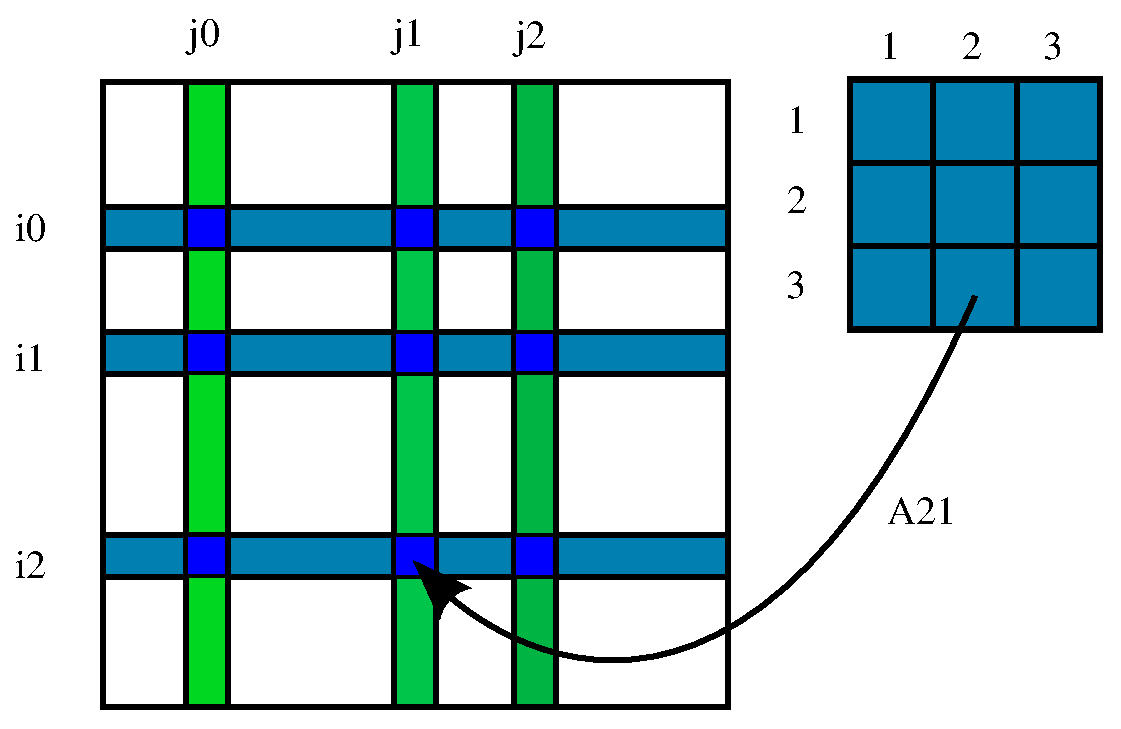
\includegraphics[height=3in]{eps/insertion.eps}
    \caption{Adding the entries of a cell tensor~$A^K$ to the
      global tensor~$A$ using the  local-to-global mapping
      $\iota_K$, illustrated here for a rank two
      tensor (a matrix).}
    \label{fig:insertion}
  \end{center}
\end{figure}

In Algorithm~\ref{alg:assembly}, we present a general algorithm for
assembling the contributions from the local cell, exterior facet and
interior facet tensors into a global sparse tensor. In
Appendix~\ref{app:assembly}, we present a sketch of the corresponding
implementation in C++ based on UFC. In both cases, we iterate over the
local cells, exterior and interior facets. On each local entity, we
compute the local tensor and add it to the global tensor as in
Figure~\ref{fig:insertion}.

\begin{algorithm}
$A = 0$ \\
\\
\emph{Assemble contributions from all cells} \\
\textbf{for each} $K \in \mathcal{T}$ \\
\\
\tab \textbf{for} $j = 1,2,\ldots,r$: \\
\tab\tab Tabulate the local-to-global mapping $\iota_K^j$ \\
\\
\tab Let $K \in \mathcal{T}_k$ \\
\tab Tabulate the cell tensor $A^K$ for $I^c_k$ \\
\tab Add $A^K_i$ to $A_{\iota_K^1(i_1), \iota_K^2(i_2), \ldots, \iota_K^r(i_r)}$ for all $i\in I_K$ \\
\\
\emph{Assemble contributions from all exterior facets} \\
\textbf{for each} $S \in \partial_e\mathcal{T}$ \\
\\
\tab \textbf{for} $j = 1,2,\ldots,r$: \\
\tab\tab Tabulate the local-to-global mapping $\iota_K^j$ \\
\\
\tab Let $S \in \partial_e\mathcal{T}_k$ \\
\tab Tabulate the exterior facet tensor $A^S$ for $I^e_k$ \\
\tab Add $A^S_i$ to $A_{\iota_K^1(i_1), \iota_K^2(i_2), \ldots, \iota_K^r(i_r)}$ for all $i\in I_K$ \\
\\
\\
\emph{Assemble contributions from all interior facets} \\
\textbf{for each} $S \in \partial_i\mathcal{T}$ \\
\\
\tab \textbf{for} $j = 1,2,\ldots,r$: \\
\tab\tab Tabulate the local-to-global mapping $\iota_K^j$ \\
\\
\tab Let $S \in \partial_i\mathcal{T}_k$ \\
\tab Tabulate the interior facet tensor $A^S$ for $I^i_k$ \\
\tab Add $A^S_i$ to $A_{\iota_K^1(i_1), \iota_K^2(i_2), \ldots, \iota_K^r(i_r)}$ for all $i\in I_K$ \\
\caption{Assembling the global tensor~$A$ from the local contributions
  on all cells, exterior and interior facets. For assembly over
  exterior facets, $K$ refers to the cell $K\in\mathcal{T}$ incident
  to the exterior facet~$S$, and for assembly over interior facets,
  $K$ refers to the ``macro cell'' consisting of the pair of cells
  $K^+$ and $K^-$ incident to the interior facet~$S$.}
\label{alg:assembly}
\end{algorithm}

\chapter{Interface specification}
\label{sec:interface}
\index{interface}

% Need to write about the Python utils somewhere, should be in appendix

\section{A short remark on design}
\index{design}

UFC is organized as a minimalistic C++ class hierarchy for
representing low-level abstractions of the finite element method. The
functions in these classes are mainly of two types: (i) Functions
returning dimensions, which are typically used to allocate an array or
check whether an existing array is of proper size and (ii) Functions
that fill an array with values according to the method and variational
form.

It is considered the user's or the assembly routine's
responsibility to allocate and deallocate arrays of proper size.
Consider for example the function for evaluating the $i$th basis
function in the class \texttt{finite\_element}:
\begin{code}
virtual void evaluate_basis(unsigned int i, double* values,
                            const double* coordinates,
                            const cell& c) const = 0;
\end{code}
This function assumes that the array \texttt{values} has the correct
size, which may be obtained by calling the functions
\texttt{value\_rank} and \texttt{value\_dimension}.

Thus, the UFC interface is a low-level interface that should be simple
to integrate into an existing C++ finite element code, but probably
not suitable to be exposed as part of an end-user interface.

The UFC interface is defined by a single header file \texttt{ufc.h}
which defines the central interface class \texttt{ufc::form} and a
small set of auxiliary interface classes. In addition a pair of data
structures \texttt{ufc::mesh} and \texttt{ufc::cell} are defined and
used for passing data to the interface functions. All functions
defined by the UFC interface are \emph{pure virtual}, meaning that
these functions must be overloaded and implemented by the user of the
interface (the form compiler generating or the programmer implementing
the UFC code). All but two functions (\texttt{init\_mesh} and
\texttt{init\_cell}) are \texttt{const}, meaning that calling these
\texttt{const} functions will leave the UFC objects unchanged.
\index{ufc.h}

The interface is presented below in the same order as it is
defined in the header file \texttt{ufc.h}. Thus, the interface is
presented bottom-up, starting with the definition of basic data
structures and ending with the definition of the \texttt{ufc::form}
interface class.

\section{Cell shapes}
\index{Cell shapes}
\index{\texttt{interval}}
\index{\texttt{triangle}}
\index{\texttt{quadrilateral}}
\index{\texttt{tetrahedron}}
\index{\texttt{hexahedron}}

\begin{code}
enum shape {interval,
            triangle,
            quadrilateral,
            tetrahedron,
            hexahedron};
\end{code}

This enumeration includes all cell shapes that are covered by the UFC
specification, see Chapter~\ref{sec:referencecells}.

\section{The class \texttt{ufc::mesh}}
\index{\texttt{ufc::mesh}}

The class \texttt{ufc::mesh} defines a data structure containing basic
information about an unstructured mesh. It is used for passing a
minimal amount of information about the global mesh to UFC functions.

\subsection{The integer \texttt{topological\_dimension}}

\begin{code}
unsigned int topological_dimension;
\end{code}

The unsigned integer \texttt{topological\_dimension} specifies the
topological dimension of the mesh, that is, the topological dimension
of the cells of the mesh. For the supported cell shapes defined above,
the topological dimensions are as follows: \texttt{interval} has
dimension one, \texttt{triangle} and \texttt{quadri\-lateral} have
dimension two, and \texttt{tetrahedron} and \texttt{hexahedron} have
dimension three.

\subsection{The integer \texttt{geometric\_dimension}}

\begin{code}
unsigned int geometric_dimension;
\end{code}

The unsigned integer \texttt{geometric\_dimension} is the geometric
dimension of the mesh, that is, the dimension of the coordinates of
the mesh vertices.  Often, the geometric dimension is equal to the
topological dimension, but they may differ. For example, one may have
a topologically two-dimensional mesh embedded in three-dimensional
space.

\subsection{The array \texttt{num\_entities}}

\begin{code}
unsigned int* num_entities;
\end{code}

The array \texttt{num\_entities} should contain the number of entities
within each topological dimension of the mesh (see
Chapter~\ref{sec:referencecells}). Thus, for a mesh of tetrahedral
cells, \texttt{num\_entities[0]} should contain the number of
vertices, \texttt{num\_entities[1]} should contain the number of edges
(if they are needed, see below), \texttt{num\_entities[2]} should
contain the number of faces, and \texttt{num\_entities[3]} should
contain the number of cells.

\section{The class \texttt{ufc::cell}}
\index{\texttt{ufc::cell}}

The class \texttt{ufc::cell} defines the data structure for a cell in
a mesh. Its intended use is not as a building block in a mesh data
structure, but merely as a view of specific data for a single cell.
It is used to pass cell data to UFC functions with a minimal amount of
assumptions on how the computational mesh is represented and stored.

\subsection{The enum variable \texttt{cell\_shape}}

\begin{code}
shape cell_shape;
\end{code}

The variable \texttt{cell\_shape} should be set to the corresponding
\texttt{ufc::shape} for the cell (see above).

\subsection{The integer \texttt{topological\_dimension}}

\begin{code}
unsigned int topological_dimension;
\end{code}

The integer \texttt{topological\_dimension} should be set equal to the
topological dimension of the cell (see above).

\subsection{The integer \texttt{geometric\_dimension}}

\begin{code}
unsigned int geometric_dimension;
\end{code}

The integer \texttt{geometric\_dimension} should be set equal to the
geometric dimension of the cell (see above).

\subsection{The array \texttt{entity\_indices}}

\begin{code}
unsigned int** entity_indices;
\end{code}

The array \texttt{entity\_indices} should contain the global indices
for all entities of the cell (see Chapter~\ref{sec:referencecells}).
The length of the array \texttt{entity\_indices} should be equal to
the value of the variable \texttt{topological\_dimension} plus one.

Thus, \texttt{entity\_indices[0]} should be an array containing the
global indices of all the vertices of the cell,
\texttt{entity\_indices[1]} should be an array containing the global
indices of all the edges of the cell, etc.

Note that the entity indices are not always needed for all entities of
the cell. The entities that are required will be specified by the
\texttt{ufc::dof\_map} class (see below).

\subsection{The array \texttt{coordinates}}

\begin{code}
double** coordinates;
\end{code}

The array \texttt{coordinates} should contain the global coordinates
for all vertices of the cell and thus its length should be equal to
number of vertices of the mesh. The length of the array
\texttt{coordinates[0]} should be equal to the value of the variable
\texttt{geometric\_dimension} and it should contain the $x$, $y$,
\ldots coordinates of the first vertex etc.

\section{The class \texttt{ufc::function}}
\index{\texttt{ufc::function}}

The class \texttt{ufc::function} is an interface for evaluation of
general tensor-valued functions on the cells of a mesh.

\begin{code}
virtual void evaluate(double* values,
                      const double* coordinates,
                      const cell& c) const = 0;
\end{code}

The only function in this class is \texttt{evaluate}, which evaluates
all the value components of the function at a given point in a given
cell of the mesh.

The output of \texttt{evaluate} should be written to the array
\texttt{values}. For a scalar-valued function, a single value should be
written to \texttt{values[0]}. For general tensor-valued functions,
the values should be written in a flattened row-major ordering of the
tensor values. Thus, for a function $f : K \rightarrow \R^2$ with $A =
f(x)$ a $2 \times 2$ matrix, the array \texttt{values} should contain
the values $A_{11}, A_{12}, A_{21}, A_{22}$.

The input to \texttt{evaluate} is the coordinates of a point in a cell
and the UFC view of the cell containing that point.

See also the description of
\texttt{ufc::finite\_element::evaluate\_dof} below.

\section{The class \texttt{ufc::finite\_element}}
\index{\texttt{ufc::finite\_element}}

The class \texttt{ufc::finite\_element} represents a finite element in
the classical Ciarlet sense~\cite{Cia78}, or rather a particular
instance of a finite element for a particular choice of nodal basis
functions. Thus, a \texttt{ufc::finite\_element} has functions for
accessing the shape of the finite element, the dimension of the
polynomial function space, the basis functions of the function space
(and their derivatives), and the linear functionals defining the
degrees of freedom. In addition, a \texttt{ufc::finite\_element}
provides functionality for interpolation.

\subsection{The function \texttt{signature}}

\begin{code}
virtual const char* signature() const = 0;
\end{code}

This function returns a signature string that uniquely identifies the
finite element. This can be used to compare whether or not two given
\texttt{ufc::fi\-nite\_element}s are identical.

\subsection{The function \texttt{cell\_shape}}

\begin{code}
virtual shape cell_shape() const = 0;
\end{code}

This function returns the shape of the cell the finite element is
defined on.

\subsection{The function \texttt{space\_dimension}}

\begin{code}
virtual unsigned int space_dimension() const = 0;
\end{code}

This function returns the dimension of the local finite element space
($|V_h^K|$), which is equal to the number of basis functions. This
should also be equal to the value of \texttt{local\_dimension()} for
the corresponding \texttt{ufc::dof\_map} (see below).

\subsection{The function \texttt{value\_rank}}

\begin{code}
virtual unsigned int value_rank() const = 0;
\end{code}

A finite element can have general tensor-valued basis functions.  The
function \texttt{value\_rank} returns the rank of the value space of
the basis functions. For a scalar element, this function should return
zero, for vector-valued functions it should return one, for
matrix-valued functions it should return two, etc.

\subsection{The function \texttt{value\_dimension}}

\begin{code}
virtual unsigned int
value_dimension(unsigned int i) const = 0;
\end{code}

This function returns the dimension of the value space of the finite
element basis functions for the given axis, where the given axis must
be a number between zero and the value rank minus one.

Note that the total size (number of values) of the value space is
obtained as the product \texttt{value\_dimension(i)} for $0 \le i <$
\texttt{value\_rank()}.

\subsection{The function \texttt{evaluate\_basis}}

\begin{code}
virtual void evaluate_basis(unsigned int i,
                            double* values,
                            const double* coordinates,
                            const cell& c) const = 0;
\end{code}

This function evaluates basis function \texttt{i} at the given
\texttt{coordinates} within the given cell \texttt{c}, and stores the
values in the array \texttt{values}. The size of this output array
equals the value size of value space (as described in the previous
section).

\subsection{The function \texttt{evaluate\_basis\_derivatives}}

\begin{code}
virtual void
evaluate_basis_derivatives(unsigned int i,
                           unsigned int n,
                           double* values,
                           const double* coordinates,
                           const ufc::cell& c) const = 0;
\end{code}

This function evaluates all order \texttt{n} derivatives of basis
function \texttt{i} at the given \texttt{coordinates} within the given
\texttt{cell}, and stores the values in the array \texttt{values}.
Derivatives may be obtained up to the polynomial degree of the finite
element function space with higher degree derivatives evaluating to
zero.

The number of derivatives is given by $d^n$ where $d$ is the geometric
dimension of the cell. For $n = 1$, $d = 3$, the order of the
derivatives is naturally $\partial/\partial x$, $\partial/\partial y$,
$\partial/\partial z$. For $n = 2$, $d = 3$, the order of the
derivatives is $\frac{\partial^2}{\partial x\partial x},
\frac{\partial^2}{\partial x\partial y}, \ldots,
\frac{\partial^2}{\partial z\partial z}$. Thus, the derivatives are
stored in a flattened row-major ordering based on the derivative
spatial dimensions.

For tensor-valued basis functions, the ordering of derivatives is
row-major based on the value space dimensions followed by the
derivative spatial dimensions.

\subsection{The function \texttt{evaluate\_dof}}

\begin{code}
virtual double evaluate_dof(unsigned int i,
                            const function& f,
                            const cell& c) const = 0;
\end{code}

This function evaluates and returns the value of the degree of freedom
\texttt{i} (which is a linear functional) on the given function
\texttt{f}.
  
For example, the degrees of freedom for Lagrange finite elements are
given by evaluation at a set of points. Other examples of degrees of
freedom include weighted integrals over facets or normal components at
facets.

\subsection{The function \texttt{interpolate\_vertex\_values}}

\begin{code}
virtual void
interpolate_vertex_values(double* vertex_values,
                          const double* dof_values,
                          const cell& c) const = 0;
\end{code}

This function takes as input the array \texttt{dof\_values} containing
the expansion coefficients for some function in the nodal basis and
computes the values of that function at the vertices of the given
cell, storing those values in the array \texttt{vertex\_values}. If
the function is tensor-valued, the values are stored in the array
\texttt{dof\_values} row-major on the list of vertices followed by the
row-major ordering of the tensor values as described above.

\subsection{The function \texttt{num\_sub\_elements}}

\begin{code}
virtual unsigned int num_sub_elements() const = 0;
\end{code}

This function returns the number of sub elements for a nested (mixed)
element. For simple elements (non-nested), this function should return
one.

A nested element is an element that is defined from a set of elements
by taking the direct sum (tensor product) of the polynomial spaces of
those elements. For example, the basis functions $\psi_1, \psi_2,
\ldots, \psi_m$ of a vector-valued Lagrange element may be constructed
from a scalar Lagrange element by repeating the basis functions
$\phi_1, \phi_2, \ldots, \phi_n$ of the scalar element and padding
with zeros: $\psi_1 = (\phi_1, 0), \psi_2 = (\phi_2, 0), \ldots,
\psi_n = (\phi_n, 0), \psi_{n+1} = (0, \phi_1), \psi_{n+2} = (0,
\phi_2), \ldots$.

Finite elements may be nested at arbitrary depth. So for example, a
mixed Taylor--Hood element may be created by combining a vector-valued
quadratic Lagrange finite element with a scalar linear Lagrange finite
element, and the vector-valued element may in turn be created by
combining a set of scalar quadratic Lagrange elements.

\subsection{The function \texttt{create\_sub\_element}}

\begin{code}
virtual finite_element*
create_sub_element(unsigned int i) const = 0;
\end{code}

This factory function constructs a \texttt{finite\_element} object for
sub element \texttt{i}. The argument \texttt{i} must be an integer
between zero and the number of sub elements
(\texttt{num\_sub\_elements}) minus one. If the element is simple
(non-nested), this function creates a copy of the finite element
itself.

\section{The class \texttt{ufc::dof\_map}}
\index{\texttt{ufc::dof\_map}}

This class represents the local-to-global mapping of degrees of
freedom (dofs), or rather one particular instance of such a mapping
(there are many possible local-to-global mappings) as defined in
\eqref{eq:iota_K}.  The most central function of this class is
\texttt{tabulate\_dofs}, which tabulates the local-to-global mapping
from the degrees of freedom on a local cell to a global vector of
degrees of freedom.

\subsection{The function \texttt{signature}}

\begin{code}
virtual const char* signature() const = 0;
\end{code}

This function returns a signature string that uniquely identifies the
finite element. This can be used to compare whether or not two given
\texttt{ufc::dof\_map}s are identical. (This may be used to optimize
the assembly of forms by caching previously computed dof maps.)

\subsection{The function \texttt{needs\_mesh\_entities}}

\begin{code}
virtual bool needs_mesh_entities(unsigned int d) const = 0;
\end{code}

This function returns true if the \texttt{dof\_map} requires mesh
entities of topological dimension \texttt{d} to be filled in
\texttt{ufc::cell} arguments. This may be used to check which entities
must be generated to tabulate the local-to-global mapping. For
example, linear Lagrange elements will only need to know the vertices
of each cell in the mesh, while quadratic Lagrange elements will also
need to know the edges (or faces) of each cell in the mesh.

\subsection{The function \texttt{init\_mesh}}

\begin{code}
virtual bool init_mesh(const mesh& mesh) = 0;
\end{code}

This function initializes the dof map for a given mesh. If it returns
true, calls to \texttt{init\_cell} and \texttt{init\_cell\_finalize}
are required to complete the initialization. The function
\texttt{global\_dimension} be may only be called when the
initialization is complete.

\subsection{The function \texttt{init\_cell}}

\begin{code}
virtual void init_cell(const mesh& m,
                       const cell& c) = 0;
\end{code}

For \texttt{dof\_map} objects where \texttt{init\_mesh} returns true,
this function must be called for each cell in the mesh to initialize
the dof mapping.

\subsection{The function \texttt{init\_cell\_finalize}}

\begin{code}
virtual void init_cell_finalize() = 0;
\end{code}

For \texttt{dof\_map} objects where \texttt{init\_mesh} returns true,
this function must be called after \texttt{init\_cell} is called for
each cell in the mesh to complete initialization of the dof mapping.

\subsection{The function \texttt{global\_dimension}}

\begin{code}
virtual unsigned int global_dimension() const = 0;
\end{code}

This function returns the dimension of the global finite element space
on the mesh that the \texttt{dof\_map} has been initialized for. The
result of calling this function before the initialization is complete
is undefined.

\subsection{The function \texttt{local\_dimension}}

\begin{code}
virtual unsigned int local_dimension() const = 0;
\end{code}

This function returns the dimension of the local finite element space
on a single cell.

\subsection{The function \texttt{num\_facet\_dofs}}

\begin{code}
virtual unsigned int num_facet_dofs() const = 0;
\end{code}

This function returns the number of dofs tied to a single facet of a
cell. This is the number of dofs that should be set if a Dirichlet
boundary condition is applied to a single facet. It is assumed that
all cells of the mesh have the same number of degrees of freedom on
each of their facets.

\subsection{The function \texttt{tabulate\_dofs}}

\begin{code}
virtual void tabulate_dofs(unsigned int* dofs,
                           const mesh& m,
                           const cell& c) const = 0;
\end{code}

This function tabulates the global dof indices corresponding to each
dof on the given cell. The size of the output array \texttt{dofs}
should be equal to the value returned by \texttt{local\_dimension()}.

\subsection{The function \texttt{tabulate\_facet\_dofs}}

\begin{code}
virtual void
tabulate_facet_dofs(unsigned int* dofs,
                    unsigned int facet) const = 0;
\end{code}

This function tabulates the local dof indices tied to a given local
facet. The size of the output array \texttt{dofs} should be equal to
the value returned by \texttt{num\_facet\_dofs()}.

\subsection{The function \texttt{tabulate\_coordinates}}

\begin{code}
virtual void tabulate_coordinates(double** coordinates,
                                  const cell& c) const = 0;
\end{code}

This function tabulates the coordinates for each dof on the given
cell. For Lagrange elements, this function will tabulate a set of
points on the given cell such that the dofs of the finite element are
given by evaluation of the function at those points.

For elements that do not have a direct relationship between
coordinates and dofs, an attempt should be made at a sensible
implementation of this function. For example, if a dof is defined as
the integral over a facet, the midpoint of the facet can be used. If
no other choice makes sense, the midpoint of the cell can be used as a
last resort. This function must thus be used with care if
non-Lagrangian elements are used.

The size of the output array \texttt{coordinates} should be equal to
the value returned by \texttt{local\_dimension()} and the size of each
sub array \texttt{coordi\-nates[0]}, \texttt{coordinates[1]} etc should
be equal to the geometric dimension of the mesh.

\subsection{The function \texttt{num\_sub\_dof\_maps}}

\begin{code}
virtual unsigned int num_sub_dof_maps() const = 0;
\end{code}

This function returns the number of sub dof maps for a nested (mixed)
element. For a discussion on the sub element concept, see the
documentation of the function
\texttt{finite\_element::num\_sub\_dof\_maps}. For simple elements
(non-nested), this function should return one.

\subsection{The function \texttt{create\_sub\_dof\_map}}

\begin{code}
virtual dof_map* create_sub_dof_map(unsigned int i) const = 0;
\end{code}

This factory function constructs a \texttt{dof\_map} object for sub
element \texttt{i}. The argument \texttt{i} must be a number between
zero and the number of sub dof maps (\texttt{num\_sub\_dof\_maps})
minus one. If the dof map is simple (non-nested), this function
creates a copy of the dof map element itself.

\section{The integral classes}

As described in Section~\ref{sec:assembly}, the global sparse tensor
(the ``stiffness matrix'') representing a given form (differential
operator) may be assembled by summing the contributions from the local
cells, exterior facets and interior facets of the mesh.

These contributions are represented in the UFC interface by the
classes \texttt{cell\_integral}, \texttt{exterior\_facet\_integral}
and \texttt{interior\_facet\_integral}. Each of these three integral
classes has a single function \texttt{tabulate\_tensor} which may be
called to compute the corresponding local contribution (cell tensor,
exterior facet tensor or interior facet tensor).

\section{The class \texttt{ufc::cell\_integral}}
\index{\texttt{ufc::cell\_integral}}

The class \texttt{ufc::cell\_integral} represents the integral of a
form over a local cell in a finite element mesh. It has a single
function \texttt{tabulate\_tensor} which may be called to tabulate the
values of the cell tensor for a given cell.

\subsection{The function \texttt{tabulate\_tensor}}
\index{\texttt{tabulate\_tensor}}

\begin{code}
virtual void tabulate_tensor(double* A,
                             const double * const * w,
                             const cell& c) const = 0;
\end{code}

This function tabulates the values of the cell tensor for a form into
the given array \texttt{A}. The size of this array should be equal to
the product of the local space dimensions for the set of finite
element function spaces corresponding to the arguments of the
form. For example, when computing the matrix for a bilinear form
defined on piecewise linear elements on triangles, the space dimension
of the local finite element is three and so the size of the array
\texttt{A} should be $3 \times 3 = 9$.

The array \texttt{w} should contain the expansion coefficients for all
\emph{coefficients} of the form in the finite element nodal basis for
each corresponding function space. Thus, the size of the array
\texttt{w} should be equal to the number of coefficients~$n$ and the
size of each each array \texttt{w[0]}, \texttt{w[1]} etc. should be
equal to the space dimension of the corresponding local finite element
space.

\subsection{The class \texttt{ufc::exterior\_facet\_integral}}
\index{\texttt{ufc::exterior\_facet\_integral}}

The class \texttt{ufc::exterior\_facet\_integral} represents the
integral of a form over a local exterior facet (boundary facet) in a
finite element mesh. It has a single function
\texttt{tabulate\_tensor} which may be called to tabulate the values
of the exterior facet tensor for a given facet.

\begin{code}
virtual void tabulate_tensor(double* A,
                             const double * const * w,
                             const cell& c,
                             unsigned int facet) const = 0;
\end{code}

The arrays \texttt{A} and \texttt{w} have the same function and should
have the same sizes as described in the documentation for
\texttt{cell\_integral::tabulate\_tensor}. Thus, the values of the
exterior facet integral will be tabulated into the array \texttt{A}
and the nodal basis expansions of all coefficients should be provided
in the array \texttt{w}.

The additional argument \texttt{facet} is required and should specify
the local number of the facet with respect to its (single) incident
cell. Thus, when the facet is an edge of a triangle, the argument
\texttt{facet} should be an integer between zero and two (0, 1, 2) and
when the facet is a facet of a tetrahedron, the argument
\texttt{facet} should be an integer between zero and three (0, 1, 2,
3).

\section{The class \texttt{ufc::interior\_facet\_integral}}
\index{\texttt{ufc::interior\_facet\_integral}}

The class \texttt{ufc::interior\_facet\_integral} represents the
integral of a form over a local interior facet in a finite element
mesh. It has a single function \texttt{tabulate\_tensor} which may be
called to tabulate the values of the interior facet tensor for a given
facet.

\subsection{The function \texttt{tabulate\_tensor}}

\begin{code}
virtual void tabulate_tensor(double* A,
                             const double * const * w,
                             const cell& c0,
                             const cell& c1,
                             unsigned int facet0,
                             unsigned int facet1) const = 0;
\end{code}

Just as for the \texttt{cell\_integral} and
\texttt{exterior\_facet\_integral} classes, the
\texttt{tabulate\_tensor} function for the class
\texttt{interior\_facet\_integral} tabulates the values of the local
(interior facet) tensor into the array \texttt{A}, given the nodal
basis expansions of the form coefficients in the array \texttt{w}.
However, the interior facet tensor contains contributions from the two
incident cells of an interior facet and thus the dimensions of these
arrays are different.

On each interior facet, the two incident (neighboring) cells form a
``macro cell'' consisting of the total set of local basis functions on
the two cells. The set of basis functions on the macro element is
obtained by extending the basis functions on each of the two cells by
zero to the macro cell. Thus, the space dimension of the finite
element function space on the macro element is twice the size of the
finite element function space on a single cell. The ordering of basis
functions and degrees of freedom on the macro cell is obtained by
first enumerating the basis functions and degrees of freedom on one of
the two cells and then the basis functions and degrees of freedom on
the second cell.

Thus the size of the array \texttt{A} should be equal to the product
of twice the local space dimensions for the set of finite element
function spaces corresponding to the arguments of the form. For
example, when computing the matrix for a bilinear form defined on
piecewise linear elements on triangles, the space dimension of the
local finite element is three and so the size of the array \texttt{A}
should be $6 \times 6 = 36$.

Similarly, the array \texttt{w} should contain the expansion
coefficients for all \emph{coefficients} of the form in the finite
element nodal basis for each corresponding function space on the macro
cell. Thus, the size of the array \texttt{w} should be equal to the
number of coefficients~$n$ and the size of each each array
\texttt{w[0]}, \texttt{w[1]} etc. should be equal to twice the space
dimension of the corresponding local finite element space.

Additional arguments \texttt{facet0} and \texttt{facet1} are required
and should specify the local number of the facet with respect to its
two incident cells. Thus, when the facet is an edge of a triangle, each
of these arguments may be an integer between zero and two (0, 1, 2)
and when the facet is a facet of a tetrahedron, each of these
arguments may be an integer between zero and three (0, 1, 2, 3).

\section{The class \texttt{ufc::form}}
\index{\texttt{ufc::form}}

The \texttt{ufc::form} class is the central part of the UFC interface
and it represents a form
\begin{equation}
  a = a(v_1, \ldots, v_r; w_1, \ldots, w_n), 
\end{equation}
defined on the product space $V_h^1 \times V_h^2 \times \cdots \times
V_h^r \times W_h^1 \times W_h^2 \times \cdots \times W_h^n$ of two
sets $\{V_h^j\}_{j=1}^r, \{W_h^j\}_{j=1}^n$ of finite element function
spaces on a triangulation $\mathcal{T}$ of a domain $\Omega \subset
\R^d$.

A \texttt{ufc::form} provides functions for accessing the rank~$r$ and
number of coefficients~$n$ for a form, and factory functions for
creating UFC objects for the corresponding cell integrals, exterior
facet integrals, interior facet integrals, and all associated finite
elements and dof maps (local-to-global mappings).

\subsection{The function \texttt{signature}}

\begin{code}
virtual const char* signature() const = 0;
\end{code}

This function returns a signature string that uniquely identifies the
form. This can be used to compare whether or not two given
\texttt{ufc::forms}s are identical.

\subsection{The function \texttt{rank}}

\begin{code}
virtual unsigned int rank() const = 0;
\end{code}

This function returns the rank~$r$ of the global tensor generated by
the form (arity of the form).

\subsection{The function \texttt{num\_coefficients}}

\begin{code}
virtual unsigned int num_coefficients() const = 0;
\end{code}

This function returns the number of coefficients~$n$ for the form.
Note that all integral terms of a form must have the same
coefficients, even if not all coefficients are present in each term of
the form.

\subsection{The function \texttt{num\_cell\_integrals}}

\begin{code}
virtual unsigned int num_cell_integrals() const = 0;
\end{code}

This function returns the number of different cell integrals for the
form. A form may have an arbitrary number of integrals over disjoint
sub domains of the mesh.

\subsection{The function \texttt{num\_exterior\_facet\_integrals}}

\begin{code}
virtual unsigned int num_exterior_facet_integrals() const = 0;
\end{code}

This function returns the number of different exterior facet integrals
for the form. A form may have an arbitrary number of integrals over
disjoint sub domains of the mesh boundary.

\subsection{The function \texttt{num\_interior\_facet\_integrals}}

\begin{code}
virtual unsigned int num_interior_facet_integrals() const = 0;
\end{code}

This function returns the number of different interior facet integrals
for the form. A form may have an arbitrary number of integrals over
disjoint subset of the interior facets of the mesh.

\subsection{The function \texttt{create\_finite\_element}}

\begin{code}
virtual finite_element*
create_finite_element(unsigned int i) const = 0;
\end{code}

This factory function constructs a \texttt{finite\_element} object for
form argument \texttt{i}. A form with rank~$r$ and a number of
coefficients~$n$ has $r + n$ arguments, so this function
returns the finite element object for tensor axis $i$ if $i < r$, or
the finite element for coefficient $i - r$ if $i \geq r$.  The caller
is responsible for deleting the returned object.

\subsection{The function \texttt{create\_dof\_map}}

\begin{code}
virtual dof_map*
create_dof_map(unsigned int i) const = 0;
\end{code}

This factory function constructs a \texttt{dof\_map} object for form
argument \texttt{i}. A form with rank~$r$ and a number of
coefficients~$n$ has $r + n$ arguments, so this function
returns the dof map object for tensor axis $i$ if $i < r$, or the dof
map for coefficient $i - r$ if $i \geq r$.  The caller is responsible
for deleting the returned object.

\subsection{The function \texttt{create\_cell\_integral}}

\begin{code}
virtual cell_integral*
create_cell_integral(unsigned int i) const = 0;
\end{code}

This factory function constructs a \texttt{cell\_integral} object for
cell domain \texttt{i}. The caller is responsible for deleting the
returned object.

\subsection{The function \texttt{create\_exterior\_facet\_integral}}

\begin{code}
virtual exterior_facet_integral*
create_exterior_facet_integral(unsigned int i) const = 0;
\end{code}

This factory function constructs an \texttt{exterior\_facet\_integral}
object for exterior facet domain \texttt{i}. The caller is responsible
for deleting the returned object.

\subsection{The function \texttt{create\_interior\_facet\_integral}}

\begin{code}
virtual interior_facet_integral*
create_interior_facet_integral(unsigned int i) const = 0;
\end{code}

This factory function constructs an \texttt{interior\_facet\_integral}
object for interior facet domain \texttt{i}. The caller is responsible
for deleting the returned object.

\chapter{Reference cells}

The definition of reference cells used in \package{} follows the
UFC specification.~\cite{www:ufc,ufcmanual}
The following five reference cells are covered by the UFC specification:
the reference \emph{interval},
the reference \emph{triangle},
the reference \emph{quadrilateral},
the reference \emph{tetrahedron} and
the reference \emph{hexahedron}.

On each of these reference cells, an \emph{ad-hoc} ordering is picked
for the vertices and the remaining entities (edges, faces, \ldots) are
ordered based on a simple rule.

\begin{table}[H]
\linespread{1.2}\selectfont
  \begin{center}
    \begin{tabular}{|l|c|c|c|}
      \hline
      Reference cell & Dimension & \#Vertices & \#Facets \\
      \hline
      \hline
      The reference interval      & 1 & 2 & 2 \\
      \hline
      The reference triangle      & 2 & 3 & 3 \\
      \hline
      The reference quadrilateral & 2 & 4 & 4 \\
      \hline
      The reference tetrahedron   & 3 & 4 & 4 \\
      \hline
      The reference hexahedron    & 3 & 8 & 6 \\
      \hline
    \end{tabular}
    \caption{Reference cells covered by the UFC specification.}
  \end{center}
\end{table}

The UFC specification assumes that each cell in a finite element mesh
is always isomorphic to one of the reference cells.

\section{Basic concepts}

\subsection{Mesh entities}

The topological entities of a cell (or mesh) are referred to as
\emph{mesh entities}. A mesh entity can be identified with a pair
$(d, i)$, where $d$ is the topological dimension of the mesh entity and $i$
is a unique index of the mesh entity. Mesh entities are numbered
within each topological dimension from $0$ to $n_d-1$, where $n_d$ is
the number of mesh entities of topological dimension $d$.

\subsection{Named mesh entities}

For convenience, mesh entities of topological dimension $0$ are
referred to as \emph{vertices}, entities of dimension $1$
as \emph{edges}, entities of dimension $2$ as \emph{faces}, entities of
\emph{codimension} $1$ as \emph{facets} and entities of codimension as
$0$ \emph{cells}. These concepts are summarized in
Table~\ref{tab:entities}.

\begin{table}[H]
\linespread{1.2}\selectfont
  \begin{center}
    \begin{tabular}{|l|c|c|}
      \hline
      Entity & Dimension & Codimension \\
      \hline
      Vertex & $0$       & -- \\
      Edge   & $1$       & -- \\
      Face   & $2$       & -- \\
      & & \\
      Facet  & --      &  $1$ \\
      Cell   & --      &  $0$ \\
      \hline
    \end{tabular}
    \caption{Named mesh entities.}
    \label{tab:entities}
  \end{center}
\end{table}

\subsection{Ordering of mesh entities}

On each reference cell, an \emph{ad-hoc} ordering is picked for its
vertices (the mesh entities of topological dimension zero). The
remaining entities are then ordered within each topological dimension
by identifying each entity with the corresponding tuple of
non-incident vertices and then ordering those tuples
lexicographically.

As an illustration, consider the ordering of edges (the mesh entities
of topological dimension one) on a triangle. In
Figure~\ref{fig:orderingexample,triangle}, the vertices of the
reference triangle are numbered counter-clockwise in the plane. The
edges of the reference triangle may then be numbered by identifying
each edge with the vertices not incident with that edge. Since there
is only one such vertex for each edge, this means that each edge is
identified with its opposite vertex. We thus identify the three edges
in the reference triangle with the tuples $(0)$, $(1)$ and $(2)$. The
first of these is edge $e_0$ between vertices $v_1$ and $v_2$ opposite
to vertex $v_0$.

Similarly, we identify the six edges of the reference tetrahedron with
the tuples $(0, 1)$, $(0, 2)$, $(0, 3)$, $(1, 2)$, $(1, 3)$ and $(2,
3)$. The first of these is edge $e_0$ between vertices $v_2$ and $v_3$
opposite to vertices $v_0$ and $v_1$ as in Figure~\ref{fig:orderingexample,tetrahedron}.

\begin{figure}[H]
  \begin{center}
    \psfrag{v0}{$v_0$}
    \psfrag{v1}{$v_1$}
    \psfrag{v2}{$v_2$}
    \psfrag{e0}{$e_0$}
    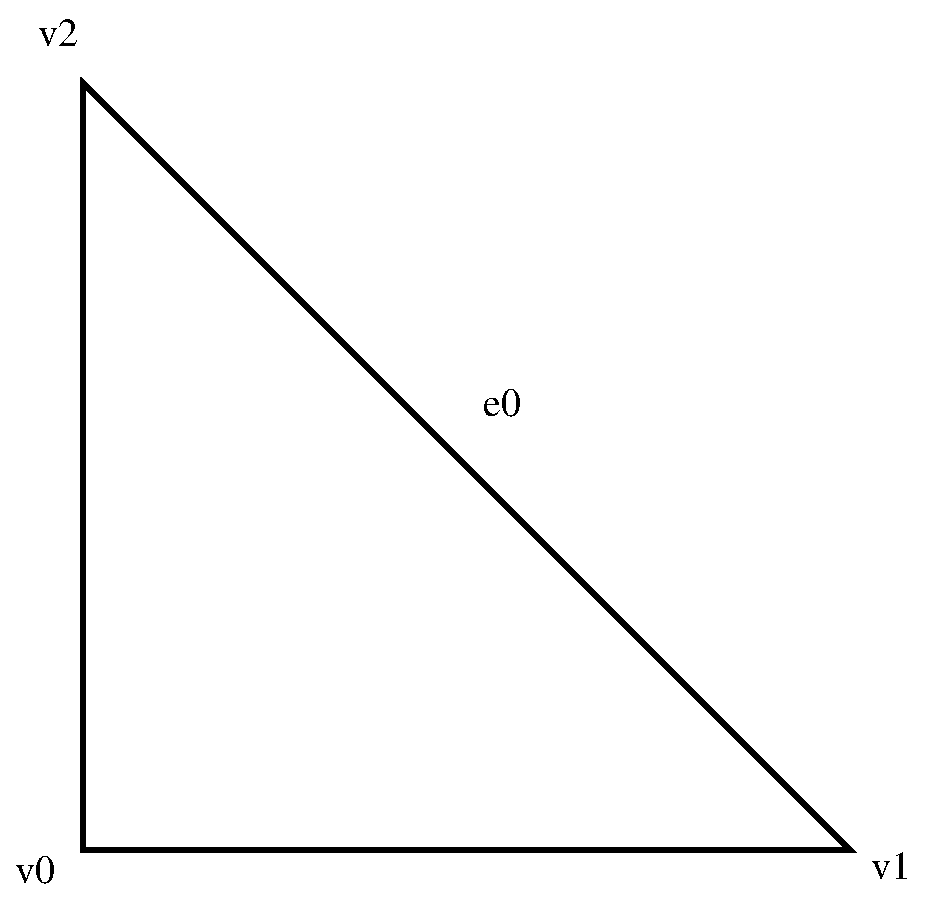
\includegraphics[width=5cm]{eps/ordering_example_triangle.eps}
    \caption{Entities are ordered based on a lexicographical ordering
      of their non-incident vertices. The first edge $e_0$ is non-incident
      with vertex $v_0$.}
    \label{fig:orderingexample,triangle}
  \end{center}
\end{figure}

\begin{figure}[H]
  \begin{center}
    \psfrag{v0}{$v_0$}
    \psfrag{v1}{$v_1$}
    \psfrag{v2}{$v_2$}
    \psfrag{v3}{$v_3$}
    \psfrag{e0}{$e_0$}
    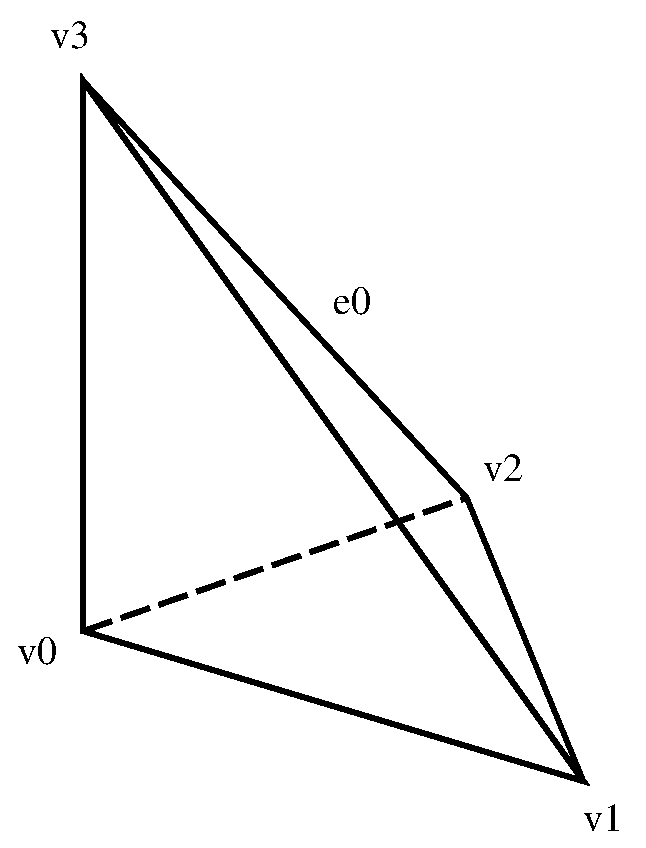
\includegraphics[width=7cm]{eps/ordering_example_tetrahedron.eps}
    \caption{Entities are ordered based on a lexicographical ordering
      of their non-incident vertices. The first edge $e_0$ is non-incident
      with vertices $v_0$ and $v_1$.}
    \label{fig:orderingexample,tetrahedron}
  \end{center}
\end{figure}

\subsection{Limitations}

The UFC specification is only concerned with the ordering of mesh
entities with respect to cells, not the ordering of mesh entities
with respect to other mesh entities of lower dimension. In other
words, the UFC specification is only concerned with the ordering of
incidence relations of the class $d - d'$ where $d$ is the
topological dimension of the mesh and $d' < d$. For example, the UFC
specification is not concerned with the ordering of incidence
relations of the class $1 - 0$, that is, the ordering of vertices on
an edge, or incidence relations of the class $2 - 1$, that is, the
ordering of edges on a face.

\newpage
\section{The reference interval}

The reference interval is shown in Figure~\ref{fig:interval} and is
defined by its two vertices with coordinates as specified in
Table~\ref{tab:interval,vertices} and mesh entities as specified in
Table~\ref{tab:interval,entities}.

\begin{figure}[H]
  \begin{center}
    \psfrag{0}{$0$}
    \psfrag{1}{$1$}
    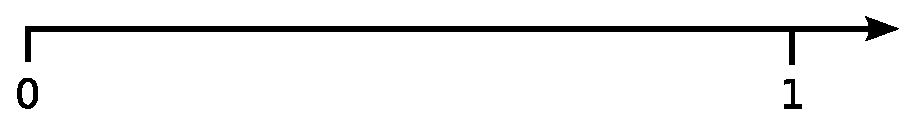
\includegraphics[width=10cm]{eps/interval.eps}
    \caption{The reference interval.}
    \label{fig:interval}
  \end{center}
\end{figure}

\begin{table}[H]
\linespread{1.2}\selectfont
  \begin{center}
    \begin{tabular}{|c|c|}
      \hline
      Vertex & Coordinate \\
      \hline
      \hline
      $v_0$ & $x = 0$ \\
      \hline
      $v_1$ & $x = 1$ \\
      \hline
    \end{tabular}
    \caption{Vertex coordinates of the reference interval.}
    \label{tab:interval,vertices}
  \end{center}
\end{table}

\begin{table}[H]
\linespread{1.2}\selectfont
  \begin{center}
    \begin{tabular}{|c|c|c|}
      \hline
      Entity & Incident vertices & Non-incident vertices \\
      \hline
      \hline
      $v_0 = (0, 0)$ & $\{v_0\}$ & $\{v_1\}$ \\
      \hline
      $v_1 = (0, 1)$ & $\{v_1\}$ & $\{v_0\}$ \\
      \hline
      $c_0 = (1, 0)$ & $\{v_0, v_1\}$ & $\emptyset$ \\
      \hline
    \end{tabular}
    \caption{Mesh entities of the reference interval.}
    \label{tab:interval,entities}
  \end{center}
\end{table}

\newpage
\section{The reference triangle}

The reference triangle is shown in Figure~\ref{fig:triangle} and is
defined by its three vertices with coordinates as specified in
Table~\ref{tab:triangle,vertices} and mesh entities as specified in
Table~\ref{tab:triangle,entities}.

\begin{figure}[H]
  \begin{center}
    \psfrag{v0}{$(0, 0)$}
    \psfrag{v1}{$(1, 0)$}
    \psfrag{v2}{$(0, 1)$}
    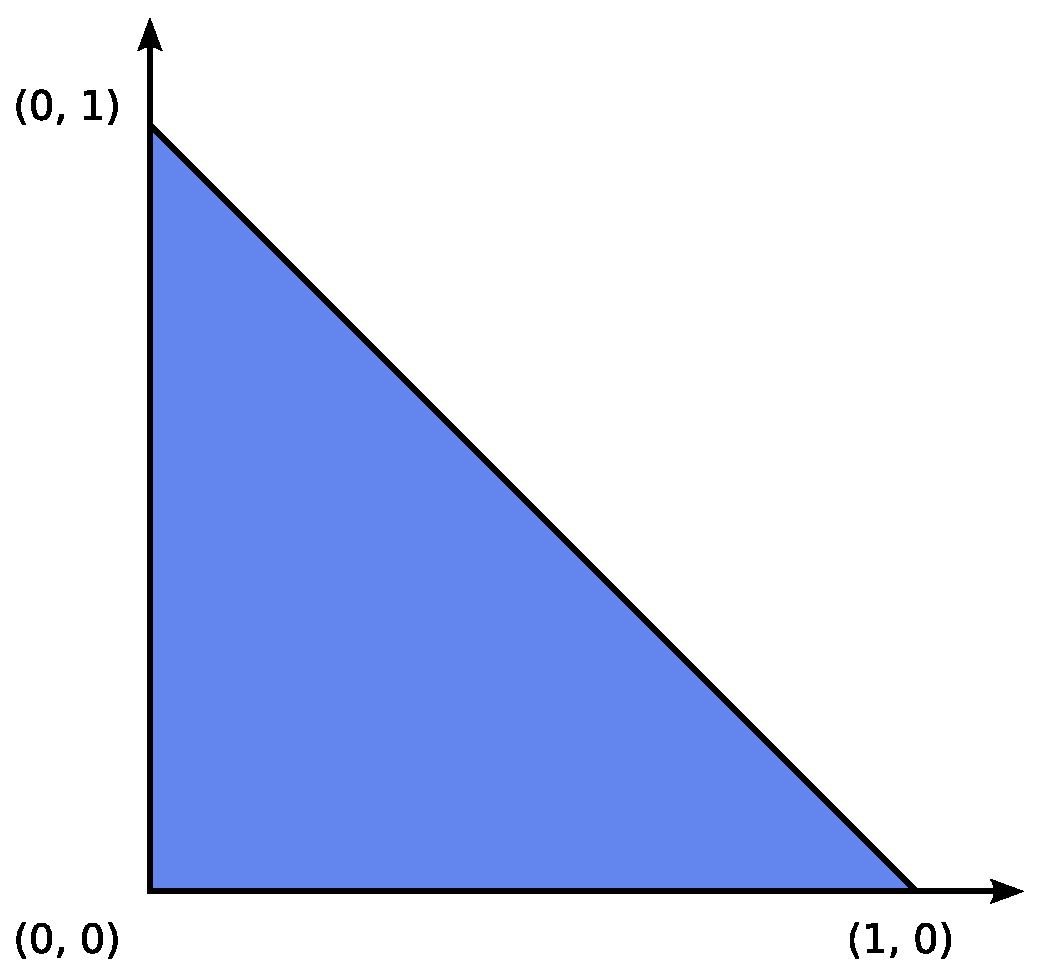
\includegraphics[width=10cm]{eps/triangle.eps}
    \caption{The reference triangle.}
    \label{fig:triangle}
  \end{center}
\end{figure}

\begin{table}[H]
\linespread{1.2}\selectfont
  \begin{center}
    \begin{tabular}{|c|c|}
      \hline
      Vertex & Coordinate \\
      \hline
      \hline
      $v_0 = (0, 0)$ & $x = (0, 0)$ \\
      \hline
      $v_1 = (0, 1)$ & $x = (1, 0)$ \\
      \hline
      $v_2 = (0, 2)$ & $x = (0, 1)$ \\
      \hline
    \end{tabular}
    \caption{Vertex coordinates of the reference triangle.}
    \label{tab:triangle,vertices}
  \end{center}
\end{table}

\begin{table}[H]
\linespread{1.2}\selectfont
  \begin{center}
    \begin{tabular}{|c|c|c|}
      \hline
      Entity & Incident vertices & Non-incident vertices \\
      \hline
      \hline
      $v_0 = (0, 0)$ & $\{v_0\}$ & $\{v_1, v_2\}$ \\
      \hline
      $v_1 = (0, 1)$ & $\{v_1\}$ & $\{v_0, v_2\}$ \\
      \hline
      $v_2 = (0, 2)$ & $\{v_2\}$ & $\{v_0, v_1\}$ \\
      \hline
      $e_0 = (1, 0)$ & $\{v_1, v_2\}$ & $\{v_0\}$ \\
      \hline
      $e_1 = (1, 1)$ & $\{v_0, v_2\}$ & $\{v_1\}$ \\
      \hline
      $e_2 = (1, 2)$ & $\{v_0, v_1\}$ & $\{v_2\}$ \\
      \hline
      $c_0 = (2, 0)$ & $\{v_0, v_1, v_2\}$ & $\emptyset$ \\
      \hline
    \end{tabular}
    \caption{Mesh entities of the reference triangle.}
    \label{tab:triangle,entities}
  \end{center}
\end{table}

\newpage
\section{The reference quadrilateral}

The reference quadrilateral is shown in Figure~\ref{fig:quadrilateral}
and is defined by its four vertices with coordinates as specified in
Table~\ref{tab:quadrilateral,vertices} and mesh entities as specified
in Table~\ref{tab:quadrilateral,entities}.

\begin{figure}[H]
  \begin{center}
    \psfrag{v0}{$(0, 0)$}
    \psfrag{v1}{$(1, 0)$}
    \psfrag{v2}{$(1, 1)$}
    \psfrag{v3}{$(0, 1)$}
    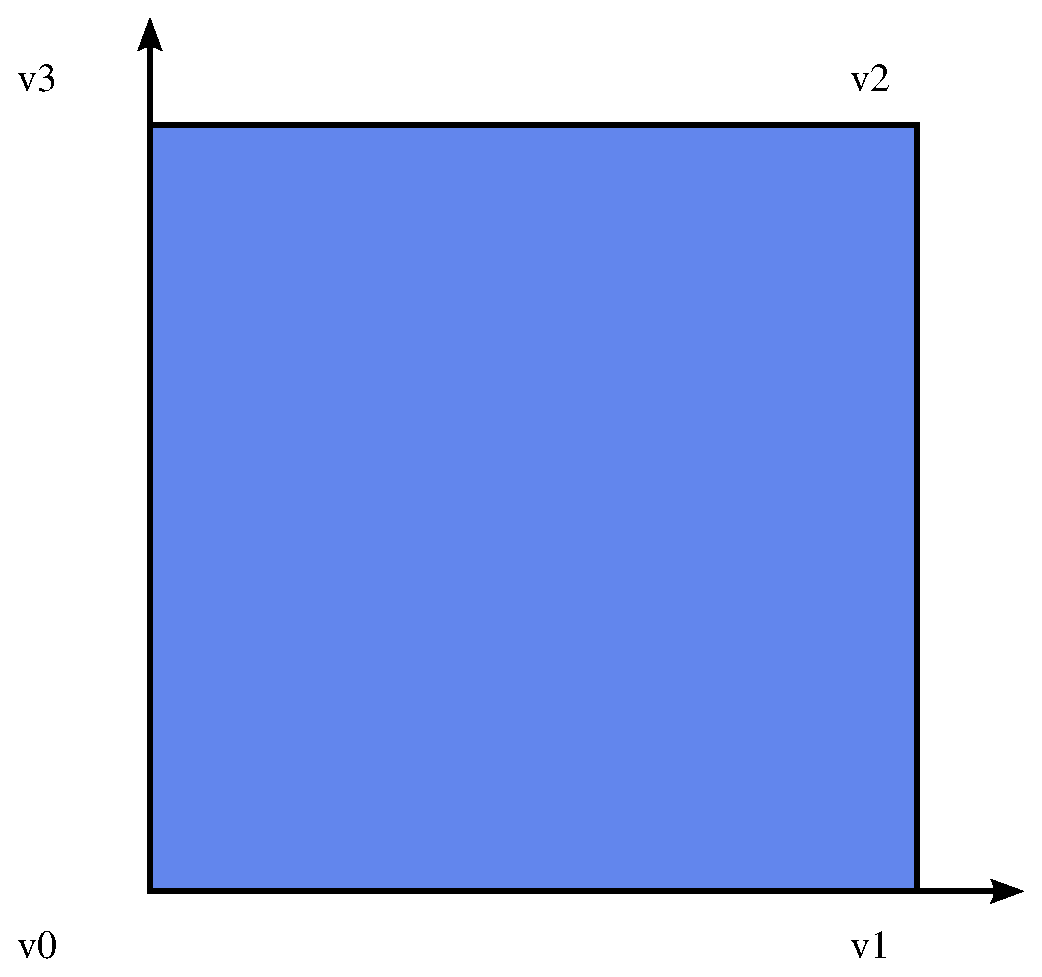
\includegraphics[width=10cm]{eps/quadrilateral.eps}
    \caption{The reference quadrilateral.}
    \label{fig:quadrilateral}
  \end{center}
\end{figure}

\begin{table}[H]
\linespread{1.2}\selectfont
  \begin{center}
    \begin{tabular}{|c|c|}
      \hline
      Vertex & Coordinate \\
      \hline
      \hline
      $v_0$ & $x = (0, 0)$ \\
      \hline
      $v_1$ & $x = (1, 0)$ \\
      \hline
      $v_2$ & $x = (1, 1)$ \\
      \hline
      $v_3$ & $x = (0, 1)$ \\
      \hline
    \end{tabular}
    \caption{Vertex coordinates of the reference quadrilateral.}
    \label{tab:quadrilateral,vertices}
  \end{center}
\end{table}

\begin{table}[H]
\linespread{1.2}\selectfont
  \begin{center}
    \begin{tabular}{|c|c|c|}
      \hline
      Entity & Incident vertices & Non-incident vertices \\
      \hline
      \hline
      $v_0 = (0, 0)$ & $\{v_0\}$ & $\{v_1, v_2, v_3\}$ \\
      \hline
      $v_1 = (0, 1)$ & $\{v_1\}$ & $\{v_0, v_2, v_3\}$ \\
      \hline
      $v_2 = (0, 2)$ & $\{v_2\}$ & $\{v_0, v_1, v_3\}$ \\
      \hline
      $v_3 = (0, 3)$ & $\{v_3\}$ & $\{v_0, v_1, v_2\}$ \\
      \hline
      $e_0 = (1, 0)$ & $\{v_2, v_3\}$ & $\{v_0, v_1\}$ \\
      \hline
      $e_1 = (1, 1)$ & $\{v_1, v_2\}$ & $\{v_0, v_3\}$ \\
      \hline
      $e_2 = (1, 2)$ & $\{v_0, v_3\}$ & $\{v_1, v_2\}$ \\
      \hline
      $e_3 = (1, 3)$ & $\{v_0, v_1\}$ & $\{v_2, v_3\}$ \\
      \hline
      $c_0 = (2, 0)$ & $\{v_0, v_1, v_2, v_3\}$ & $\emptyset$ \\
      \hline
    \end{tabular}
    \caption{Mesh entities of the reference quadrilateral.}
    \label{tab:quadrilateral,entities}
  \end{center}
\end{table}

\newpage
\section{The reference tetrahedron}

The reference tetrahedron is shown in Figure~\ref{fig:tetrahedron} and
is defined by its four vertices with coordinates as specified in
Table~\ref{tab:tetrahedron,vertices} and mesh entities as specified in
Table~\ref{tab:tetrahedron,entities}.

\begin{figure}[H]
  \begin{center}
    \psfrag{v0}{$(0, 0, 0)$}
    \psfrag{v1}{$(1, 0, 0)$}
    \psfrag{v2}{$(0, 1, 0)$}
    \psfrag{v3}{$(0, 0, 1)$}
    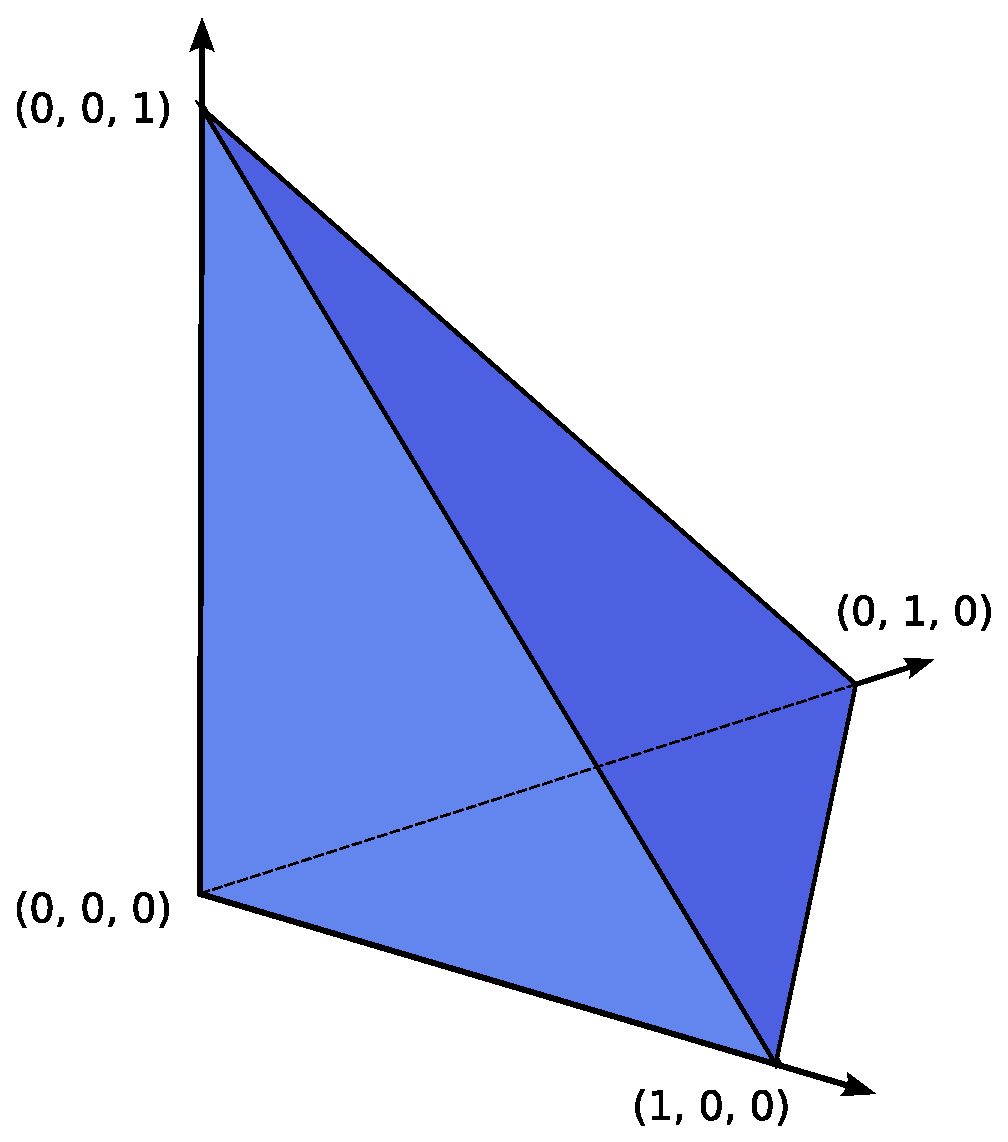
\includegraphics[width=10cm]{eps/tetrahedron.eps}
    \caption{The reference tetrahedron.}
    \label{fig:tetrahedron}
  \end{center}
\end{figure}

\begin{table}[H]
\linespread{1.2}\selectfont
  \begin{center}
    \begin{tabular}{|c|c|}
      \hline
      Vertex & Coordinate \\
      \hline
      \hline
      $v_0$ & $x = (0, 0, 0)$ \\
      \hline
      $v_1$ & $x = (1, 0, 0)$ \\
      \hline
      $v_2$ & $x = (0, 1, 0)$ \\
      \hline
      $v_3$ & $x = (0, 0, 1)$ \\
      \hline
    \end{tabular}
    \caption{Vertex coordinates of the reference tetrahedron.}
    \label{tab:tetrahedron,vertices}
  \end{center}
\end{table}

\begin{table}[H]
\linespread{1.2}\selectfont
  \begin{center}
    \begin{tabular}{|c|c|c|}
      \hline
      Entity & Incident vertices & Non-incident vertices \\
      \hline
      \hline
      $v_0 = (0, 0)$ & $\{v_0\}$ & $\{v_1, v_2, v_3\}$ \\
      \hline
      $v_1 = (0, 1)$ & $\{v_1\}$ & $\{v_0, v_2, v_3\}$ \\
      \hline
      $v_2 = (0, 2)$ & $\{v_2\}$ & $\{v_0, v_1, v_3\}$ \\
      \hline
      $v_3 = (0, 3)$ & $\{v_3\}$ & $\{v_0, v_1, v_2\}$ \\
      \hline
      $e_0 = (1, 0)$ & $\{v_2, v_3\}$ & $\{v_0, v_1\}$ \\
      \hline
      $e_1 = (1, 1)$ & $\{v_1, v_3\}$ & $\{v_0, v_2\}$ \\
      \hline
      $e_2 = (1, 2)$ & $\{v_1, v_2\}$ & $\{v_0, v_3\}$ \\
      \hline
      $e_3 = (1, 3)$ & $\{v_0, v_3\}$ & $\{v_1, v_2\}$ \\
      \hline
      $e_4 = (1, 4)$ & $\{v_0, v_2\}$ & $\{v_1, v_3\}$ \\
      \hline
      $e_5 = (1, 5)$ & $\{v_0, v_1\}$ & $\{v_2, v_3\}$ \\
      \hline
      $f_0 = (2, 0)$ & $\{v_1, v_2, v_3\}$ & $\{v_0\}$ \\
      \hline
      $f_1 = (2, 1)$ & $\{v_0, v_2, v_3\}$ & $\{v_1\}$ \\
      \hline
      $f_2 = (2, 2)$ & $\{v_0, v_1, v_3\}$ & $\{v_2\}$ \\
      \hline
      $f_3 = (2, 3)$ & $\{v_0, v_1, v_2\}$ & $\{v_3\}$ \\
      \hline
      $c_0 = (3, 0)$ & $\{v_0, v_1, v_2, v_3\}$ & $\emptyset$ \\
      \hline
    \end{tabular}
    \caption{Mesh entities of the reference tetrahedron.}
        \label{tab:tetrahedron,entities} 
  \end{center}
\end{table}

\newpage
\section{The reference hexahedron}

The reference hexahedron is shown in Figure~\ref{fig:hexahedron} and
is defined by its eight vertices with coordinates as specified in
Table~\ref{tab:hexahedron,vertices} and mesh entities as specified in
Table~\ref{tab:hexahedron,entities}.

\begin{figure}[H]
\linespread{1.2}\selectfont
  \begin{center}
    \psfrag{v0}{$(0, 0, 0)$}
    \psfrag{v1}{$(1, 0, 0)$}
    \psfrag{v2}{$(1, 1, 0)$}
    \psfrag{v3}{$(0, 1, 0)$}
    \psfrag{v4}{$(0, 0, 1)$}
    \psfrag{v5}{$(1, 0, 1)$}
    \psfrag{v6}{$(1, 1, 1)$}
    \psfrag{v7}{$(0, 1, 1)$}
    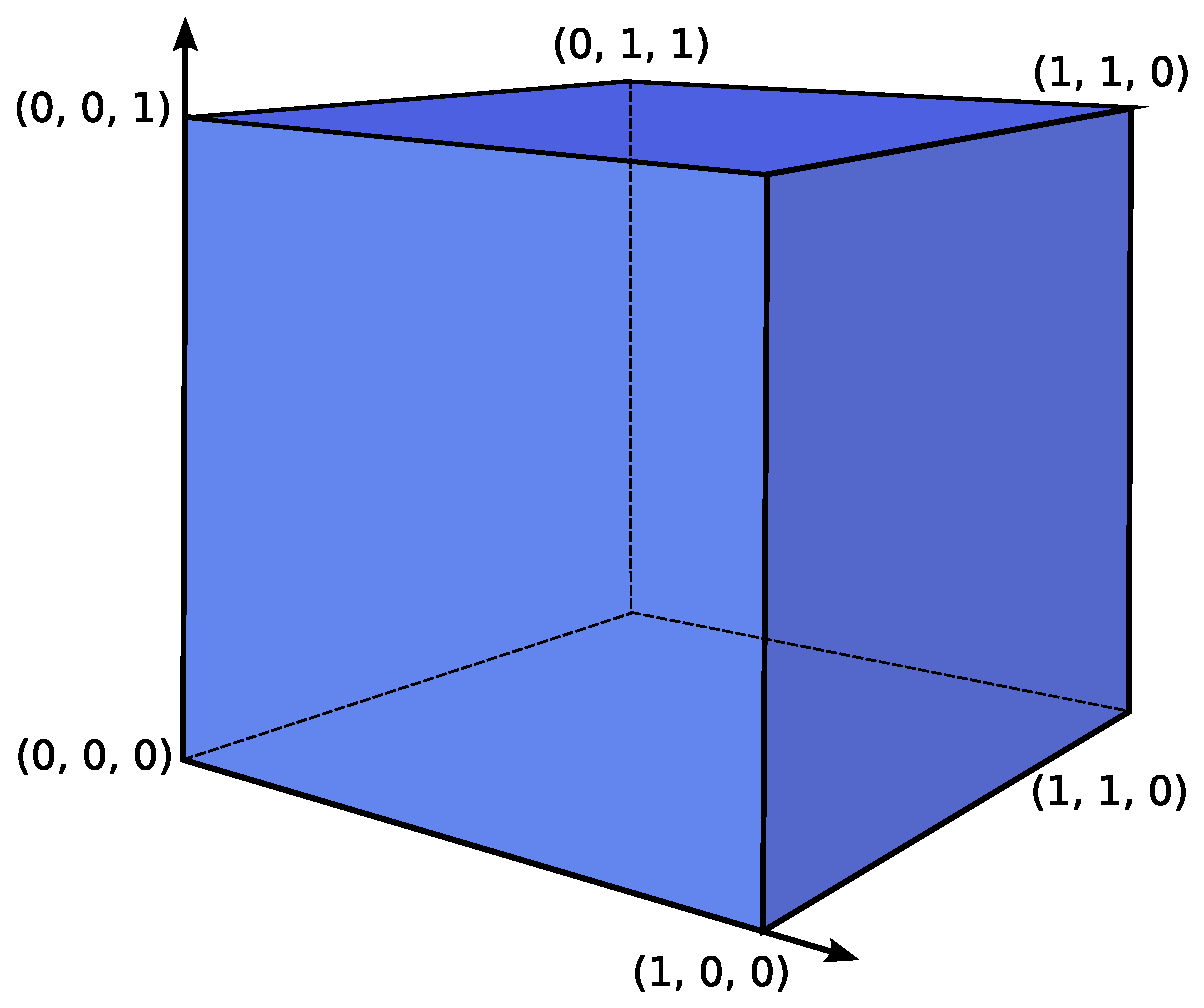
\includegraphics[width=10cm]{eps/hexahedron.eps}
    \caption{The reference hexahedron.}
    \label{fig:hexahedron}
  \end{center}
\end{figure}

\begin{table}[H]
\linespread{1.2}\selectfont
  \begin{center}
    \begin{tabular}{|c|c|}
      \hline
      Vertex & Coordinate \\
      \hline
      \hline
      $v_0$ & $x = (0, 0, 0)$ \\
      \hline
      $v_1$ & $x = (1, 0, 0)$ \\
      \hline
      $v_2$ & $x = (1, 1, 0)$ \\
      \hline
      $v_3$ & $x = (0, 1, 0)$ \\
      \hline
      $v_4$ & $x = (0, 0, 1)$ \\
      \hline
      $v_5$ & $x = (1, 0, 1)$ \\
      \hline
      $v_6$ & $x = (1, 1, 1)$ \\
      \hline
      $v_7$ & $x = (0, 1, 1)$ \\
      \hline
    \end{tabular}
    \caption{Vertex coordinates of the reference hexahedron.}
    \label{tab:hexahedron,vertices}
  \end{center}
\end{table}

\begin{table}[H]
\linespread{1.2}\selectfont
  \begin{center}
    \begin{tabular}{|c|c|c|}
      \hline
      Entity & Incident vertices & Non-incident vertices \\
      \hline
      \hline
      $v_0 = (0, 0)$ & $\{v_0\}$ & $\{v_1, v_2, v_3, v_4, v_5, v_6, v_7\}$ \\
      \hline
      $v_1 = (0, 1)$ & $\{v_1\}$ & $\{v_0, v_2, v_3, v_4, v_5, v_6, v_7\}$ \\
      \hline
      $v_2 = (0, 2)$ & $\{v_2\}$ & $\{v_0, v_1, v_3, v_4, v_5, v_6, v_7\}$ \\
      \hline
      $v_3 = (0, 3)$ & $\{v_3\}$ & $\{v_0, v_1, v_2, v_4, v_5, v_6, v_7\}$ \\
      \hline
      $v_4 = (0, 4)$ & $\{v_4\}$ & $\{v_0, v_1, v_2, v_3, v_5, v_6, v_7\}$ \\
      \hline
      $v_5 = (0, 5)$ & $\{v_5\}$ & $\{v_0, v_1, v_2, v_3, v_4, v_6, v_7\}$ \\
      \hline
      $v_6 = (0, 6)$ & $\{v_6\}$ & $\{v_0, v_1, v_2, v_3, v_4, v_5, v_7\}$ \\
      \hline
      $v_7 = (0, 7)$ & $\{v_7\}$ & $\{v_0, v_1, v_2, v_3, v_4, v_5, v_6\}$ \\
      \hline
      $e_0 = (1, 0)$ & $\{v_6, v_7\}$ & $\{v_0, v_1, v_2, v_3, v_4, v_5\}$ \\
      \hline
      $e_1 = (1, 1)$ & $\{v_5, v_6\}$ & $\{v_0, v_1, v_2, v_3, v_4, v_7\}$ \\
      \hline
      $e_2 = (1, 2)$ & $\{v_4, v_7\}$ & $\{v_0, v_1, v_2, v_3, v_5, v_6\}$ \\
      \hline
      $e_3 = (1, 3)$ & $\{v_4, v_5\}$ & $\{v_0, v_1, v_2, v_3, v_6, v_7\}$ \\
      \hline
      $e_4 = (1, 4)$ & $\{v_3, v_7\}$ & $\{v_0, v_1, v_2, v_4, v_5, v_6\}$ \\
      \hline
      $e_5 = (1, 5)$ & $\{v_2, v_6\}$ & $\{v_0, v_1, v_3, v_4, v_5, v_7\}$ \\
      \hline
      $e_6 = (1, 6)$ & $\{v_2, v_3\}$ & $\{v_0, v_1, v_4, v_5, v_6, v_7\}$ \\
      \hline
      $e_7 = (1, 7)$ & $\{v_1, v_5\}$ & $\{v_0, v_2, v_3, v_4, v_6, v_7\}$ \\
      \hline
      $e_8 = (1, 8)$ & $\{v_1, v_2\}$ & $\{v_0, v_3, v_4, v_5, v_6, v_7\}$ \\
      \hline
      $e_9 = (1, 9)$ & $\{v_0, v_4\}$ & $\{v_1, v_2, v_3, v_5, v_6, v_7\}$ \\
      \hline
      $e_{10} = (1, 10)$ & $\{v_0, v_3\}$ & $\{v_1, v_2, v_4, v_5, v_6, v_7\}$ \\
      \hline
      $e_{11} = (1, 11)$ & $\{v_0, v_1\}$ & $\{v_2, v_3, v_4, v_5, v_6, v_7\}$ \\
      \hline
      $f_0 = (2, 0)$ & $\{v_4, v_5, v_6, v_7\}$ & $\{v_0, v_1, v_2, v_3\}$ \\
      \hline
      $f_1 = (2, 1)$ & $\{v_2, v_3, v_6, v_7\}$ & $\{v_0, v_1, v_4, v_5\}$ \\
      \hline
      $f_2 = (2, 2)$ & $\{v_1, v_2, v_5, v_6\}$ & $\{v_0, v_3, v_4, v_7\}$ \\
      \hline
      $f_3 = (2, 3)$ & $\{v_0, v_3, v_4, v_7\}$ & $\{v_1, v_2, v_5, v_6\}$ \\
      \hline
      $f_4 = (2, 4)$ & $\{v_0, v_1, v_4, v_5\}$ & $\{v_2, v_3, v_6, v_7\}$ \\
      \hline
      $f_5 = (2, 5)$ & $\{v_0, v_1, v_2, v_3\}$ & $\{v_4, v_5, v_6, v_7\}$ \\
      \hline
      $c_0 = (3, 0)$ & $\{v_0, v_1, v_2, v_3, v_4, v_5, v_6, v_7\}$ & $\emptyset$ \\
      \hline
    \end{tabular}
    \caption{Mesh entities of the reference hexahedron.}
    \label{tab:hexahedron,entities}
  \end{center}
\end{table}


\chapter{Numbering of mesh entities}
\label{sec:numbering}

\index{numbering}

The UFC specification dictates a certain numbering of the vertices,
edges etc. of the cells of a finite element mesh. First, an \emph{ad
hoc} numbering is picked for the vertices of each cell. Then, the
remaining entities are ordered based on a simple rule, as described in
detail below.

\section{Basic concepts}
\index{mesh entity}
\index{topological dimension}

The topological entities of a cell (or mesh) are referred to as
\emph{mesh entities}. A mesh entity can be identified by a pair
$(d, i)$, where $d$ is the topological dimension of the mesh entity and $i$
is a unique index of the mesh entity. Mesh entities are numbered
within each topological dimension from $0$ to $n_d-1$, where $n_d$ is
the number of mesh entities of topological dimension $d$.

For convenience, mesh entities of topological dimension $0$ are
referred to as \emph{vertices}, entities of dimension $1$
as \emph{edges}, entities of dimension $2$ as \emph{faces}, entities of
\emph{codimension} $1$ as \emph{facets} and entities of codimension
$0$ as \emph{cells}. These concepts are summarized in
Table~\ref{tab:entities}.

Thus, the vertices of a tetrahedron are identified as
$v_0 = (0, 0)$, $v_1 = (0, 1)$ and $v_2 = (0, 2)$,
the edges are
$e_0 = (1, 0)$, $e_1 = (1, 1)$, $e_2 = (1, 2)$,
$e_3 = (1, 3)$, $e_4 = (1, 4)$ and $e_5 = (1, 5)$,
the faces (facets) are
$f_0 = (2, 0)$, $f_1 = (2, 1)$, $f_2 = (2, 2)$ and $f_3 = (2, 3)$,
and the cell itself is
$c_0 = (3, 0)$.

\begin{table}
\linespread{1.2}\selectfont
  \begin{center}
    \begin{tabular}{|l|c|c|}
      \hline
      Entity & Dimension & Codimension \\
      \hline
      Vertex & $0$       & -- \\
      Edge   & $1$       & -- \\
      Face   & $2$       & -- \\
      & & \\
      Facet  & --      &  $1$ \\
      Cell   & --      &  $0$ \\
      \hline
    \end{tabular}
    \caption{Named mesh entities.}
    \label{tab:entities}
  \end{center}
\end{table}

\section{Numbering of vertices}
\index{vertex numbering}

For simplicial cells (intervals, triangles and tetrahedra) of a finite
element mesh, the vertices are numbered locally based on the
corresponding global vertex numbers. In particular, a tuple of
increasing local vertex numbers corresponds to a tuple of increasing
global vertex numbers.  This is illustrated in
Figure~\ref{fig:numbering_example_triangles} for a mesh consisting of
two triangles.
 
\begin{figure}[htbp]
  \begin{center}
    \psfrag{v0}{$v_0$}
    \psfrag{v1}{$v_1$}
    \psfrag{v2}{$v_2$}
    \psfrag{0}{$0$}
    \psfrag{1}{$1$}
    \psfrag{2}{$2$}
    \psfrag{3}{$3$}
    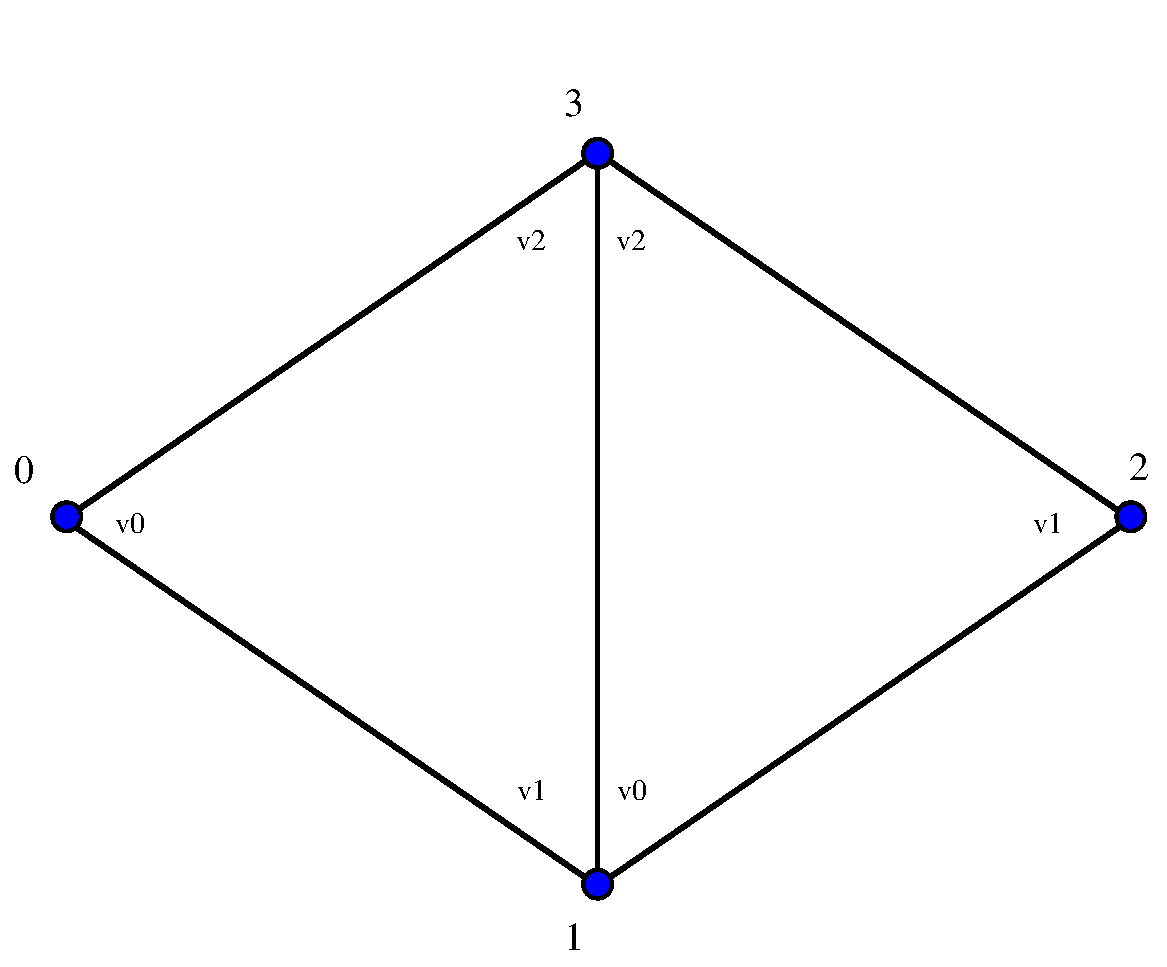
\includegraphics[width=8cm]{eps/numbering_example_triangles.eps}
    \caption{The vertices of a simplicial mesh are numbered locally
      based on the corresponding global vertex numbers.}
    \label{fig:numbering_example_triangles}
  \end{center}
\end{figure}

For non-simplicial cells (quadrilaterals and hexahedra), the numbering
is arbitrary, as long as each cell is isomorphic to the corresponding
reference cell by matching each vertex with the corresponding vertex
in the reference cell. This is illustrated in
Figure~\ref{fig:numbering_example_quadrilaterals} for a mesh
consisting of two quadrilaterals.

\begin{figure}[htbp]
  \begin{center}
    \psfrag{v0}{$v_0$}
    \psfrag{v1}{$v_1$}
    \psfrag{v2}{$v_2$}
    \psfrag{v3}{$v_3$}
    \psfrag{0}{$0$}
    \psfrag{1}{$1$}
    \psfrag{2}{$2$}
    \psfrag{3}{$3$}
    \psfrag{4}{$4$}
    \psfrag{5}{$5$}
    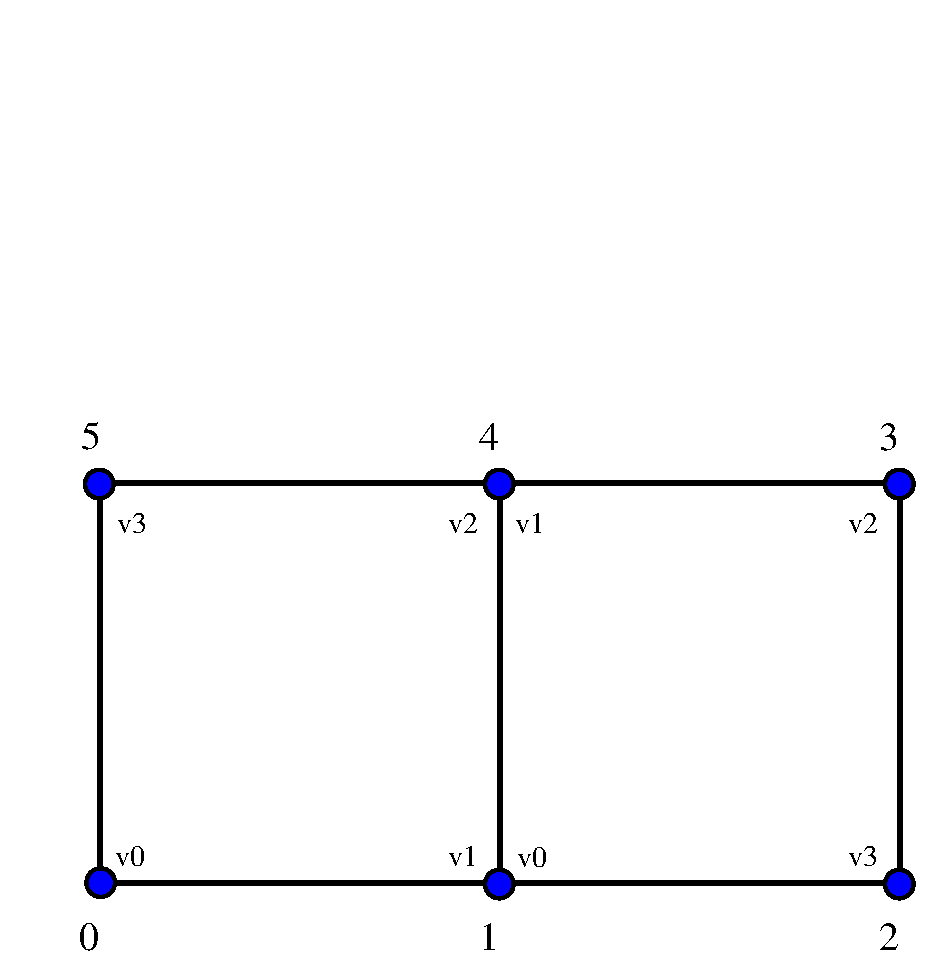
\includegraphics[width=8cm]{eps/numbering_example_quadrilaterals.eps}
    \caption{The local numbering of vertices of a non-simplicial mesh
      is arbitrary, as long as each cell is isomorphic to the
      reference cell by matching each vertex to the corresponding
      vertex of the reference cell.}
    \label{fig:numbering_example_quadrilaterals}
  \end{center}
\end{figure}

\section{Numbering of other mesh entities}

When the vertices have been numbered, the remaining mesh entities are
numbered within each topological dimension based on a
\emph{lexicographical ordering} of the corresponding ordered tuples of
\emph{non-incident vertices}.

As an illustration, consider the numbering of edges (the mesh entities
of topological dimension one) on the reference triangle in
Figure~\ref{fig:orderingexample,triangle}. To number the edges of the
reference triangle, we identify for each edge the corresponding
non-incident vertices. For each edge, there is only one such vertex
(the vertex opposite to the edge). We thus identify the three edges in
the reference triangle with the tuples $(v_0)$, $(v_1)$ and $(v_2)$. The
first of these is edge $e_0$ between vertices $v_1$ and $v_2$ opposite
to vertex $v_0$, the second is edge $e_1$ between vertices $v_0$ and
$v_2$ opposite to vertex $v_1$, and the third is edge $e_2$ between
vertices $v_0$ and $v_1$ opposite to vertex $v_2$.

Similarly, we identify the six edges of the reference tetrahedron with
the corresponding non-incident tuples $(v_0, v_1)$, $(v_0, v_2)$,
$(v_0, v_3)$, $(v_1, v_2)$, $(v_1, v_3)$ and $(v_2, v_3)$. The first of these is
edge $e_0$ between vertices $v_2$ and $v_3$ opposite to vertices $v_0$
and $v_1$ as shown in Figure~\ref{fig:orderingexample,tetrahedron}.

\begin{figure}[htbp]
  \begin{center}
    \psfrag{v0}{$v_0$}
    \psfrag{v1}{$v_1$}
    \psfrag{v2}{$v_2$}
    \psfrag{e0}{$e_0$}
    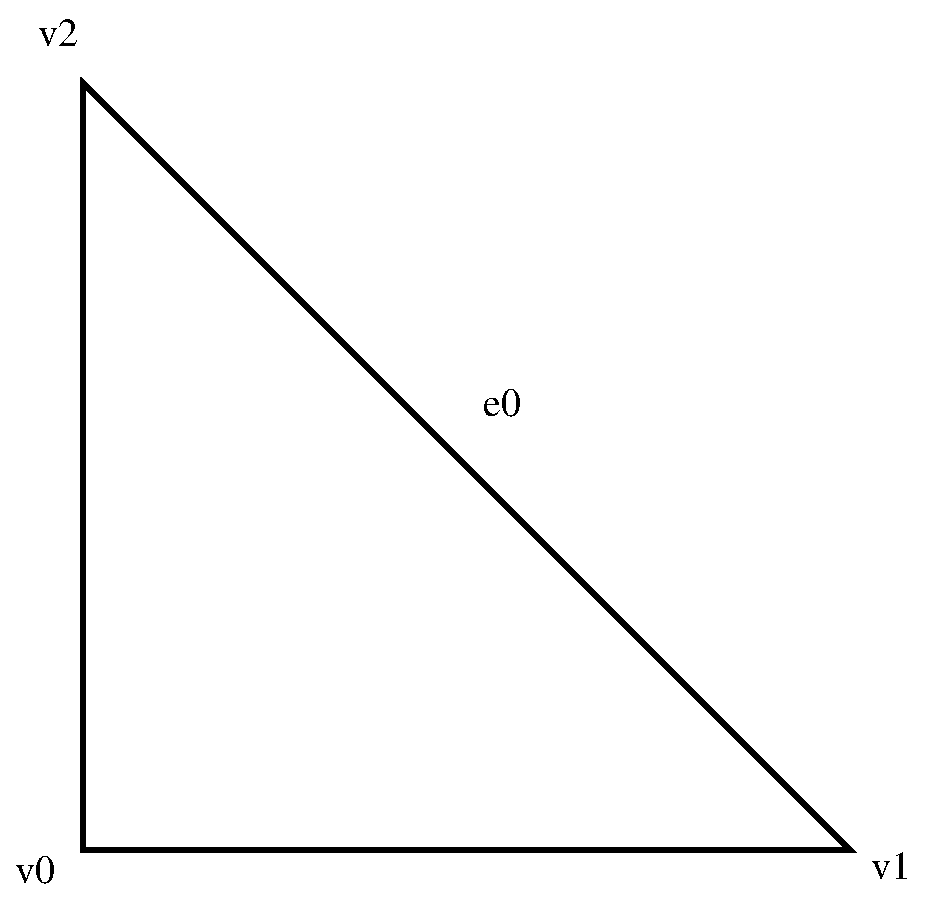
\includegraphics[width=5cm]{eps/ordering_example_triangle.eps}
    \caption{Mesh entities are ordered based on a lexicographical ordering
      of the corresponding ordered tuples of non-incident vertices.
      The first edge $e_0$ is non-incident to vertex $v_0$.}
    \label{fig:orderingexample,triangle}
  \end{center}
\end{figure}

\begin{figure}[htbp]
  \begin{center}
    \psfrag{v0}{$v_0$}
    \psfrag{v1}{$v_1$}
    \psfrag{v2}{$v_2$}
    \psfrag{v3}{$v_3$}
    \psfrag{e0}{$e_0$}
    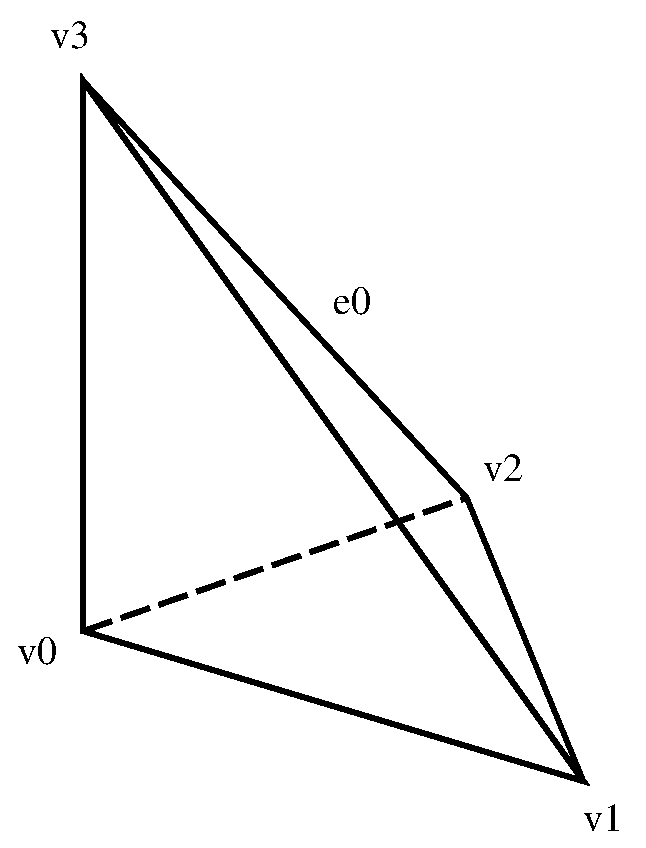
\includegraphics[width=5cm]{eps/ordering_example_tetrahedron.eps}
    \caption{Mesh entities are ordered based on a lexicographical ordering
      of the corresponding ordered tuples of non-incident vertices.
      The first edge $e_0$ is non-incident to vertices $v_0$ and $v_1$.}
    \label{fig:orderingexample,tetrahedron}
  \end{center}
\end{figure}

\subsection{Relative ordering}

The relative ordering of mesh entities with respect to other incident
mesh entities follows by sorting the entities by their (global)
indices. Thus, the pair of vertices incident to the first edge $e_0$
of a triangular cell is $(v_1, v_2)$, not $(v_2, v_1)$. Similarly, the
first face $f_0$ of a tetrahedral cell is incident to vertices $(v_1,
v_2, v_3)$.

For simplicial cells, the relative ordering in combination with the
convention of numbering the vertices locally based on global vertex
indices means that two incident cells will always agree on the
orientation of incident subsimplices. Thus, two incident triangles
will agree on the orientation of the common edge and two incident
tetrahedra will agree on the orientation of the common edge(s) and the
orientation of the common face (if any). This is illustrated in
Figure~\ref{fig:orientation_example_triangles} for two incident
triangles sharing a common edge.

\begin{figure}[htbp]
  \begin{center}
    \psfrag{v0}{$v_0$}
    \psfrag{v1}{$v_1$}
    \psfrag{v2}{$v_2$}
    \psfrag{v3}{$v_3$}
    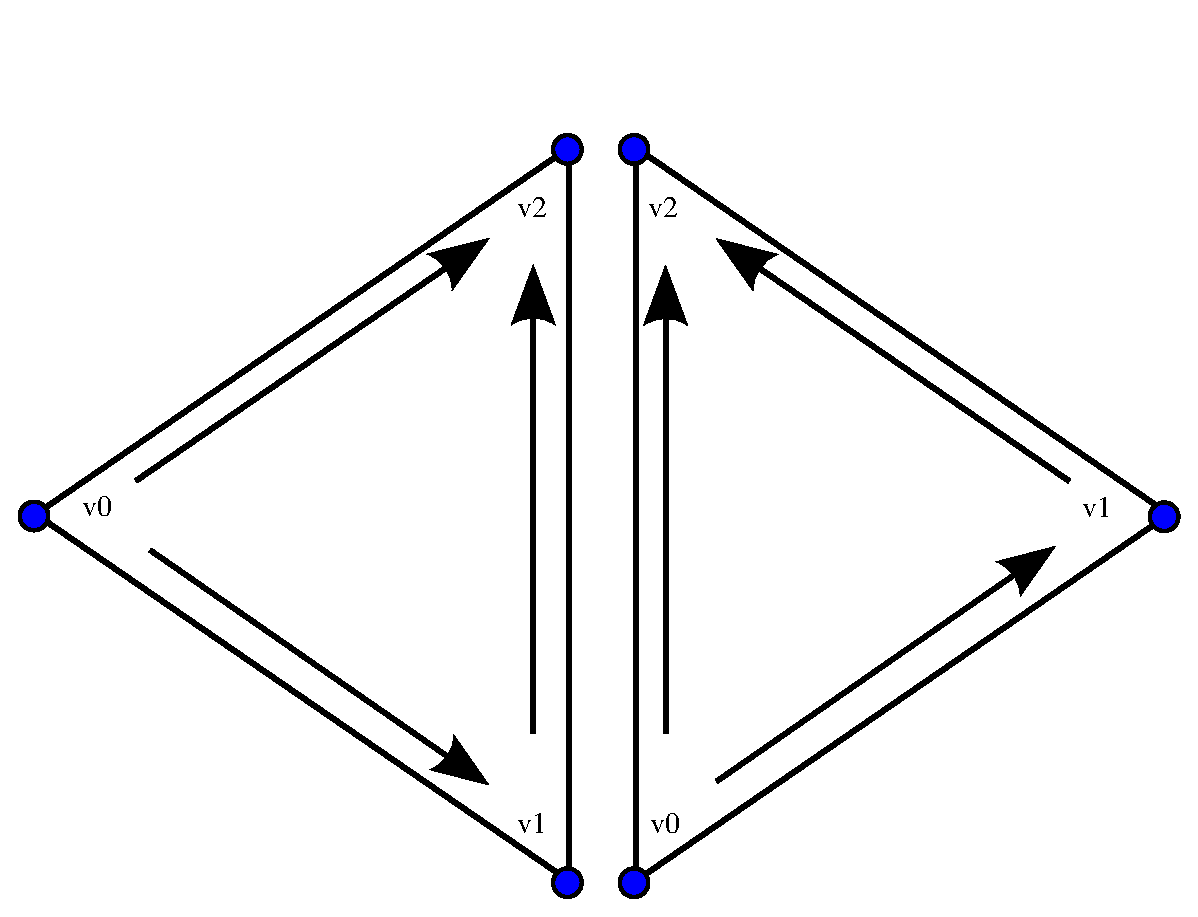
\includegraphics[width=9cm]{eps/orientation_example_triangles.eps}
    \caption{Two incident triangles will always agree on the
      orientation of the common edge.}
    \label{fig:orientation_example_triangles}
  \end{center}
\end{figure}

\subsection{Limitations}
 
The UFC specification is only concerned with the ordering of mesh
entities with respect to entities of larger topological dimension. In
other words, the UFC specification is only concerned with the ordering
of incidence relations of the class $d - d'$ where $d > d'$. For
example, the UFC specification is not concerned with the ordering of
incidence relations of the class $0 - 1$, that is, the ordering of
edges incident to vertices.

\newpage

\section{Numbering schemes for reference cells}

The numbering scheme is demonstrated below for cells
isomorphic to each of the five reference cells.

\subsection{Numbering of mesh entities on intervals}

\begin{minipage}{\textwidth}
\linespread{1.2}\selectfont
  \begin{center}
    \begin{tabular}{|c|c|c|}
      \hline
      Entity & Incident vertices & Non-incident vertices \\
      \hline
      \hline
      $v_0 = (0, 0)$ & $(v_0)$ & $(v_1)$ \\
      \hline
      $v_1 = (0, 1)$ & $(v_1)$ & $(v_0)$ \\
      \hline
      $c_0 = (1, 0)$ & $(v_0, v_1)$ & $\emptyset$ \\
      \hline
    \end{tabular}
  \end{center}
\end{minipage}

\subsection{Numbering of mesh entities on triangular cells}
%
\begin{minipage}{\textwidth}
\linespread{1.2}\selectfont
  \begin{center}
    \begin{tabular}{|c|c|c|}
      \hline
      Entity & Incident vertices & Non-incident vertices \\
      \hline
      \hline
      $v_0 = (0, 0)$ & $(v_0)$ & $(v_1, v_2)$ \\
      \hline
      $v_1 = (0, 1)$ & $(v_1)$ & $(v_0, v_2)$ \\
      \hline
      $v_2 = (0, 2)$ & $(v_2)$ & $(v_0, v_1)$ \\
      \hline
      $e_0 = (1, 0)$ & $(v_1, v_2)$ & $(v_0)$ \\
      \hline
      $e_1 = (1, 1)$ & $(v_0, v_2)$ & $(v_1)$ \\
      \hline
      $e_2 = (1, 2)$ & $(v_0, v_1)$ & $(v_2)$ \\
      \hline
      $c_0 = (2, 0)$ & $(v_0, v_1, v_2)$ & $\emptyset$ \\
      \hline
    \end{tabular}
  \end{center}
\end{minipage}

\subsection{Numbering of mesh entities on quadrilateral cells}
%
\begin{minipage}{\textwidth}
\linespread{1.1}\selectfont
  \begin{center}
    \begin{tabular}{|c|c|c|}
      \hline
      Entity & Incident vertices & Non-incident vertices \\
      \hline
      \hline
      $v_0 = (0, 0)$ & $(v_0)$ & $(v_1, v_2, v_3)$ \\
      \hline
      $v_1 = (0, 1)$ & $(v_1)$ & $(v_0, v_2, v_3)$ \\
      \hline
      $v_2 = (0, 2)$ & $(v_2)$ & $(v_0, v_1, v_3)$ \\
      \hline
      $v_3 = (0, 3)$ & $(v_3)$ & $(v_0, v_1, v_2)$ \\
      \hline
      $e_0 = (1, 0)$ & $(v_2, v_3)$ & $(v_0, v_1)$ \\
      \hline
      $e_1 = (1, 1)$ & $(v_1, v_2)$ & $(v_0, v_3)$ \\
      \hline
      $e_2 = (1, 2)$ & $(v_0, v_3)$ & $(v_1, v_2)$ \\
      \hline
      $e_3 = (1, 3)$ & $(v_0, v_1)$ & $(v_2, v_3)$ \\
      \hline
      $c_0 = (2, 0)$ & $(v_0, v_1, v_2, v_3)$ & $\emptyset$ \\
      \hline
    \end{tabular}
  \end{center}
\end{minipage}


\subsection{Numbering of mesh entities on tetrahedral cells}
%
\begin{minipage}{\textwidth}
\linespread{1.1}\selectfont
  \begin{center}
    \begin{tabular}{|c|c|c|}
      \hline
      Entity & Incident vertices & Non-incident vertices \\
      \hline
      \hline
      $v_0 = (0, 0)$ & $(v_0)$ & $(v_1, v_2, v_3)$ \\
      \hline
      $v_1 = (0, 1)$ & $(v_1)$ & $(v_0, v_2, v_3)$ \\
      \hline
      $v_2 = (0, 2)$ & $(v_2)$ & $(v_0, v_1, v_3)$ \\
      \hline
      $v_3 = (0, 3)$ & $(v_3)$ & $(v_0, v_1, v_2)$ \\
      \hline
      $e_0 = (1, 0)$ & $(v_2, v_3)$ & $(v_0, v_1)$ \\
      \hline
      $e_1 = (1, 1)$ & $(v_1, v_3)$ & $(v_0, v_2)$ \\
      \hline
      $e_2 = (1, 2)$ & $(v_1, v_2)$ & $(v_0, v_3)$ \\
      \hline
      $e_3 = (1, 3)$ & $(v_0, v_3)$ & $(v_1, v_2)$ \\
      \hline
      $e_4 = (1, 4)$ & $(v_0, v_2)$ & $(v_1, v_3)$ \\
      \hline
      $e_5 = (1, 5)$ & $(v_0, v_1)$ & $(v_2, v_3)$ \\
      \hline
      $f_0 = (2, 0)$ & $(v_1, v_2, v_3)$ & $(v_0)$ \\
      \hline
      $f_1 = (2, 1)$ & $(v_0, v_2, v_3)$ & $(v_1)$ \\
      \hline
      $f_2 = (2, 2)$ & $(v_0, v_1, v_3)$ & $(v_2)$ \\
      \hline
      $f_3 = (2, 3)$ & $(v_0, v_1, v_2)$ & $(v_3)$ \\
      \hline
      $c_0 = (3, 0)$ & $(v_0, v_1, v_2, v_3)$ & $\emptyset$ \\
      \hline
    \end{tabular}
  \end{center}
\end{minipage}

\vfill

\newpage

\subsection{Numbering of mesh entities on hexahedral cells}

\begin{minipage}{\textwidth}
\small
\linespread{1.2}\selectfont
  \begin{center}
    \begin{tabular}{|c|c|c|}
      \hline
      Entity & Incident vertices & Non-incident vertices \\
      \hline
      \hline
      $v_0 = (0, 0)$ & $(v_0)$ & $(v_1, v_2, v_3, v_4, v_5, v_6, v_7)$ \\
      \hline
      $v_1 = (0, 1)$ & $(v_1)$ & $(v_0, v_2, v_3, v_4, v_5, v_6, v_7)$ \\
      \hline
      $v_2 = (0, 2)$ & $(v_2)$ & $(v_0, v_1, v_3, v_4, v_5, v_6, v_7)$ \\
      \hline
      $v_3 = (0, 3)$ & $(v_3)$ & $(v_0, v_1, v_2, v_4, v_5, v_6, v_7)$ \\
      \hline
      $v_4 = (0, 4)$ & $(v_4)$ & $(v_0, v_1, v_2, v_3, v_5, v_6, v_7)$ \\
      \hline
      $v_5 = (0, 5)$ & $(v_5)$ & $(v_0, v_1, v_2, v_3, v_4, v_6, v_7)$ \\
      \hline
      $v_6 = (0, 6)$ & $(v_6)$ & $(v_0, v_1, v_2, v_3, v_4, v_5, v_7)$ \\
      \hline
      $v_7 = (0, 7)$ & $(v_7)$ & $(v_0, v_1, v_2, v_3, v_4, v_5, v_6)$ \\
      \hline
      $e_0 = (1, 0)$ & $(v_6, v_7)$ & $(v_0, v_1, v_2, v_3, v_4, v_5)$ \\
      \hline
      $e_1 = (1, 1)$ & $(v_5, v_6)$ & $(v_0, v_1, v_2, v_3, v_4, v_7)$ \\
      \hline
      $e_2 = (1, 2)$ & $(v_4, v_7)$ & $(v_0, v_1, v_2, v_3, v_5, v_6)$ \\
      \hline
      $e_3 = (1, 3)$ & $(v_4, v_5)$ & $(v_0, v_1, v_2, v_3, v_6, v_7)$ \\
      \hline
      $e_4 = (1, 4)$ & $(v_3, v_7)$ & $(v_0, v_1, v_2, v_4, v_5, v_6)$ \\
      \hline
      $e_5 = (1, 5)$ & $(v_2, v_6)$ & $(v_0, v_1, v_3, v_4, v_5, v_7)$ \\
      \hline
      $e_6 = (1, 6)$ & $(v_2, v_3)$ & $(v_0, v_1, v_4, v_5, v_6, v_7)$ \\
      \hline
      $e_7 = (1, 7)$ & $(v_1, v_5)$ & $(v_0, v_2, v_3, v_4, v_6, v_7)$ \\
      \hline
      $e_8 = (1, 8)$ & $(v_1, v_2)$ & $(v_0, v_3, v_4, v_5, v_6, v_7)$ \\
      \hline
      $e_9 = (1, 9)$ & $(v_0, v_4)$ & $(v_1, v_2, v_3, v_5, v_6, v_7)$ \\
      \hline
      $e_{10} = (1, 10)$ & $(v_0, v_3)$ & $(v_1, v_2, v_4, v_5, v_6, v_7)$ \\
      \hline
      $e_{11} = (1, 11)$ & $(v_0, v_1)$ & $(v_2, v_3, v_4, v_5, v_6, v_7)$ \\
      \hline
      $f_0 = (2, 0)$ & $(v_4, v_5, v_6, v_7)$ & $(v_0, v_1, v_2, v_3)$ \\
      \hline
      $f_1 = (2, 1)$ & $(v_2, v_3, v_6, v_7)$ & $(v_0, v_1, v_4, v_5)$ \\
      \hline
      $f_2 = (2, 2)$ & $(v_1, v_2, v_5, v_6)$ & $(v_0, v_3, v_4, v_7)$ \\
      \hline
      $f_3 = (2, 3)$ & $(v_0, v_3, v_4, v_7)$ & $(v_1, v_2, v_5, v_6)$ \\
      \hline
      $f_4 = (2, 4)$ & $(v_0, v_1, v_4, v_5)$ & $(v_2, v_3, v_6, v_7)$ \\
      \hline
      $f_5 = (2, 5)$ & $(v_0, v_1, v_2, v_3)$ & $(v_4, v_5, v_6, v_7)$ \\
      \hline
      $c_0 = (3, 0)$ & $(v_0, v_1, v_2, v_3, v_4, v_5, v_6, v_7)$ & $\emptyset$ \\
      \hline
    \end{tabular}
  \end{center}
\end{minipage}




\newpage
\bibliographystyle{siam}
\bibliography{bibliography}

\appendix

\chapter{C++ Interface}

Below follows a verbatim copy of the complete UFC interface which is
specified in the header file~\texttt{ufc.h}.

\scriptsize
\VerbatimInput[frame=single,rulecolor=\color{blue}]{code/ufc.h}
\normalsize

\chapter{A basic UFC-based assembler}
\label{app:assembly}

Below, we include a sketch of a UFC-based implementation of the assembly
of the global tensor~$A$ by summing the local contributions from all
cells. The contributions from all exterior and interior facets may be
computed similarly.

The implementation is incomplete and system specific details such as
interaction with mesh and linear algebra libraries have been
omitted.\footnote{For an example of a complete implementation of a
UFC-based assembler, we refer to the source code of
DOLFIN~\cite{www:dolfin}, in particular class \texttt{Assembler} as
implemented in \texttt{Assembler.cpp}.}

\scriptsize
\begin{code}
void assemble(..., ufc::form& form, ...)
{
  ...

  // Initialize mesh data structure
  ufc::mesh mesh;
  mesh.num_entities = new unsigned int[...];
  ...

  // Initialize cell data structure
  ufc::cell cell;
  cell.entity_indices = new unsigned int[...];
  cell.coordinates = new double[...];
  ...

  // Create cell integrals
  ufc::cell_integral** cell_integrals;
  cell_integrals = new ufc::cell_integral*[form.num_cell_integrals()];
  for (unsigned int i = 0; i < form.num_cell_integrals(); i++)
    cell_integrals[i] = form.create_cell_integral(i);

  // Create dofmaps
  ufc::dofmaps** dofmaps;
  dofmaps = new ufc::dofmap*[form.rank() + form.num_coefficients()];
  for (unsigned int i = 0; i < form.rank() + form.num_coefficients(); i++)
  {
    dofmaps[i] = form.create_dofmap(i);

    // Initialize dofmap
    if (dofmaps[i]->init_mesh(mesh))
    {
      // Iterate over cells
      for (...)
      {
        // Update cell data structure to current cell
        cell.entity_indices[...] = ...
        cell.coordinates[...] = ...
        ...

        // Initialize dofmap for cell
        dofmaps[i]->init_cell(mesh, cell);
      }

      dofmap.init_cell_finalize();
    }
  }

  // Initialize array of values for the cell tensor
  unsigned int size = 1;
  for (unsigned int i = 0; i < form.rank(); i++)
    size *= dofmaps[i]->max_local_dimension();
  double* AK = new double[size];

  // Initialize array of local to global dofmaps
  unsigned int** dofs = new unsigned int*[form.rank()];
  for (unsigned int i = 0; i < form.rank(); i++)
    dofs[i] = new unsigned int[dofmaps[i]->max_local_dimension()];

  // Initialize array of coefficient values
  double** w = new double*[form.num_coefficients()];
  for (unsigned int i = 0; i < form.num_coefficients(); i++)
    w[i] = new double[dofmaps[form.rank() + i]->max_local_dimension()];

  // Iterate over cells
  for (...)
  {
    // Get number of subdomain for current cell
    const unsigned int sub_domain = ...

    // Update cell data structure to current cell
    cell.entity_indices[...] = ...
    cell.coordinates[...] = ...
    ...

    // Interpolate coefficients (library specific so omitted here)
    ...

    // Tabulate dofs for each dimension
    for (unsigned int i = 0; i < ufc.form.rank(); i++)
      dofmaps[i]->tabulate_dofs(dofs[i], mesh, cell);

    // Tabulate cell tensor
    cell_integrals[sub_domain]->tabulate_tensor(AK, w, cell);

    // Add entries to global tensor (library specific so omitted here)
    ...
  }

  // Delete data structures
  delete [] mesh.num_entities;
  ...
}
\end{code}
\normalsize

\chapter{Complete UFC code for Poisson's equation}
\index{Poisson's equation}
\index{example code}

In this section, a simple example is given of UFC code generated by
the form compilers
FFC~\cite{www:ffc,logg:article:07,logg:article:09,logg:article:10,logg:article:11}
and SyFi~\cite{www:syfi} for Poisson's equation. The code presented
below is generated for the bilinear form of Poisson's equation for
standard continuous piecewise linear Lagrange finite elements on a
two-dimensional domain $\Omega$,
\begin{equation}
  a(v, u) = \int_{\Omega} \nabla v \cdot \nabla u \dx.
\end{equation}

Although FFC and SyFi are two different form compilers, with very
different approaches to code generation, both generate code that
conforms to the UFC specification and may thus be used interchangeably
within any UFC-based system.

In the generated code, we have omitted the two functions
\texttt{evaluate\_basis} and
\texttt{evaluate\_basis\_derivatives}\footnotemark{} to save space.

\footnotetext{For FFC, this may be done by using the compiler flags
  \texttt{-fno-evaluate\_basis} and
  \texttt{-fno-evaluate\_basis\_derivatives}.}

\section{Code generated by FFC}
\index{FFC}

\scriptsize
\VerbatimInput[frame=single,rulecolor=\color{blue}]{code/poisson_ffc.h}
\normalsize

\section{Code generated by SyFi}
\index{SyFi}

In the following we list the complete code for the finite element, 
the dofmap and the variational form for computing a stiffness matrix
based on linear Lagrangian elements in 2D. 

The code below is generated for the assembler in PyCC and it therefore
includes some PyCC files, since the option \texttt{SFC.options.include\_from = "pycc"} was used during the code generation. If PyCC is not present, the option \texttt{SFC.options.include\_from = "syfi"} can be used, and this will result in some additional files that define the numbering scheme.    

\subsection{Header file for linear Lagrange element in 2D}

\scriptsize
\VerbatimInput[frame=single,rulecolor=\color{blue}]{code/stiffness_syfi/fe_Lagrange_1_2D.h}
\normalsize

\subsection{Source file for linear Lagrange element in 2D}
\scriptsize
\VerbatimInput[frame=single,rulecolor=\color{blue}]{code/stiffness_syfi/fe_Lagrange_1_2D.cpp}
\normalsize

\subsection{Header file for the dofmap}
\scriptsize
\VerbatimInput[frame=single,rulecolor=\color{blue}]{code/stiffness_syfi/dof_map_Lagrange_1_2D.h}
\normalsize

\subsection{Source file for the dofmap}
\scriptsize
\VerbatimInput[frame=single,rulecolor=\color{blue}]{code/stiffness_syfi/dof_map_Lagrange_1_2D.cpp}
\normalsize

\subsection{Header file for the stiffness matrix form}
\scriptsize
\VerbatimInput[frame=single,rulecolor=\color{blue}]{code/stiffness_syfi/form__stiffness_form__Lagrange_1_2D.h}
\normalsize


\subsection{Source file for the stiffness matrix form}
\scriptsize
\VerbatimInput[frame=single,rulecolor=\color{blue}]{code/stiffness_syfi/form__stiffness_form__Lagrange_1_2D.cpp}
\normalsize

\chapter{Python utilities}
\index{Python utilities}
\index{code generation}

The UFC distribution includes a set of Python utilities for generating
code that conforms to the UFC specification. These utilities consist
of format string templates for C++ header files (\texttt{.h} files),
implementation files (\texttt{.cpp}) and combined header and
implementation files (\texttt{.h} files containing both the
declaration and definition of the UFC functions).

The following format strings are provided:

\begin{code}
function_combined_{header, implementation, combined}
finite_element_{header, implementation, combined}
dof_map_{header, implementation, combined}
cell_integral_{header, implementation, combined}
exterior_facet_integral_{header, implementation, combined}
interior_facet_integral_{header, implementation, combined}
form_{header, implementation, combined}
\end{code}

We demonstrate below how to use the format string
\texttt{form\_combined} together with a dictionary that specifies the
code to be inserted into the format string. Typically, a form compiler
will first generate the code to be inserted into the dictionary and
then in a later stage write the generated code to file in UFC format
using the provided format strings.

\begin{code}
from ufc import form_combined

code = {}
code["classname"] = "Poisson",
...
code["rank"] = "    return 2;",
code["num_coefficients"] = "    return 0;",
code["num_cell_integrals"] = "    return 1;",
...

print form_combined % code
\end{code}

\chapter{Installation}
\label{app:installation}
\index{installation}

\newcommand{\ufc}{UFC}

The \ufc{} package consists of two parts, the main part being a single header file called ufc.h.
In addition we have provided a set of Python utilities to simplify the generation of \ufc{} compliant code.

%The package is portable and should work on any system with a standard Python installation.
Questions, bug reports and patches concerning
the installation should be directed to the
\ufc{} mailing list at the address
\begin{code}
ufc-dev@fenics.org
\end{code}

\ufc{} must currently be installed directly from source, but Debian
(Ubuntu) packages will be available in the future, for \ufc{} and
other \fenics{} components.

%------------------------------------------------------------------------------

\section{Installing from source}

\subsection{Dependencies and requirements}
\index{dependencies}

The installation system is based on distutils, and should work on any system with a standard Python installation.

\subsubsection{Installing Python}

If Python is not installed on your system, it can be downloaded from
\begin{code}
http://www.python.org/
\end{code}
Follow the installation instructions for Python given on the Python web page.
For Debian (Ubuntu) users, the package to install is named \texttt{python}.

\subsection{Installing \ufc{}}

\ufc{} follows the standard installation procedure for Python
packages. Enter the source directory of \ufc{} and issue the
following command:
\begin{code}
# python setup.py install
\end{code}
This will install the \ufc{} utility Python package in a subdirectory
called \texttt{ufc} in the default location for user-installed Python
packages (usually something like \texttt{/usr/lib/python2.5/site-packages}).
In addition, the compiler executable (a Python script) will be
installed in the default directory for user-installed Python scripts
(usually in \texttt{/usr/bin}).

To see a list of optional parameters to the installation script, type
\begin{code}
# python setup.py install --help
\end{code}
If you don't have root access to the system you are using, you can
pass the \texttt{--home} option to the installation script to install
\ufc{} in your home directory:
\begin{code}
# mkdir ~/local
# python setup.py install --home ~/local
\end{code}
This installs the \ufc{} package in the directory \texttt{\~{}/local/lib/python}.
If you use this option, make sure to set the environment variable \texttt{PYTHONPATH}
to \texttt{\~{}/local/lib/python} and to add \texttt{\~{}/local/bin}
to the \texttt{PATH} environment variable.


%------------------------------------------------------------------------------
\section{Debian (Ubuntu) package}
\index{Debian package}
%\index{Ubuntu package}

Debian packages for simpler installation of \fenics{} packages are in preparation and will be available in the future.


\chapter{License}
\index{license}

The UFC specification, and in particular the header file
\texttt{ufc.h}, is released into the public domain.


\end{document}
